%%%%%%%%%%%%%%%%%%%%%%%%%%%%%%%%%%%%%%%%%
% Masters/Doctoral Thesis 
% LaTeX Template
% Version 2.5 (27/8/17)
%
% This template was downloaded from:
% http://www.LaTeXTemplates.com
%
% Version 2.x major modifications by:
% Vel (vel@latextemplates.com)
%
% This template is based on a template by:
% Steve Gunn (http://users.ecs.soton.ac.uk/srg/softwaretools/document/templates/)
% Sunil Patel (http://www.sunilpatel.co.uk/thesis-template/)
%
% Template license:
% CC BY-NC-SA 3.0 (http://creativecommons.org/licenses/by-nc-sa/3.0/)
%
%%%%%%%%%%%%%%%%%%%%%%%%%%%%%%%%%%%%%%%%%

%----------------------------------------------------------------------------------------
%	PACKAGES AND OTHER DOCUMENT CONFIGURATIONS
%----------------------------------------------------------------------------------------

\documentclass[
11pt, % The default document font size, options: 10pt, 11pt, 12pt
%oneside, % Two side (alternating margins) for binding by default, uncomment to switch to one side
spanish, % ngerman for German
singlespacing, % Single line spacing, alternatives: onehalfspacing or doublespacing
%draft, % Uncomment to enable draft mode (no pictures, no links, overfull hboxes indicated)
%nolistspacing, % If the document is onehalfspacing or doublespacing, uncomment this to set spacing in lists to single
%liststotoc, % Uncomment to add the list of figures/tables/etc to the table of contents
%toctotoc, % Uncomment to add the main table of contents to the table of contents
%parskip, % Uncomment to add space between paragraphs
%nohyperref, % Uncomment to not load the hyperref package
headsepline, % Uncomment to get a line under the header
% chapterinoneline, % Uncomment to place the chapter title next to the number on one line
% consistentlayout, % Uncomment to change the layout of the declaration, abstract and acknowledgements pages to \textit{match} the default layout
]{MastersDoctoralThesis} % The class file specifying the document structure

\usepackage[utf8]{inputenc} % Required for inputting international characters
\usepackage[T1]{fontenc} % Output font encoding for international characters

\usepackage{mathpazo} % Use the Palatino font by default
\usepackage{graphicx}
\usepackage[backend=bibtex,bibencoding=ascii,style=numeric,natbib=true]{biblatex} % Use the bibtex backend with the authoryear citation style (which resembles APA)

\addbibresource{example.bib} % The filename of the bibliography

\usepackage[autostyle=true]{csquotes} % Required to generate language-dependent quotes in the bibliography
\usepackage{float}
% \usepackage{tabu}
\usepackage{booktabs}
% \usepackage[table,xcdraw]{xcolor}

%----------------------------------------------------------------------------------------
%	MARGIN SETTINGS
%----------------------------------------------------------------------------------------

\geometry{
	paper=a4paper, % Change to letterpaper for US letter
	outer=2.5cm, % Inner margin
	inner=3.8cm, % Outer margin
	bindingoffset=.5cm, % Binding offset
	top=1.5cm, % Top margin
	bottom=1.5cm, % Bottom margin
	%showframe, % Uncomment to show how the type block is set on the page
}

%----------------------------------------------------------------------------------------
%	THESIS INFORMATION
%----------------------------------------------------------------------------------------

\thesistitle{Distribución de Contenido Administrado por SDN} % Your thesis title, this is used in the title and abstract, print it elsewhere with \ttitle
\supervisor{Ing. Hugo \textsc{Carrer}} % Your supervisor's name, this is used in the title page, print it elsewhere with \supname
\examiner{Dr. Ing. Mario Rafael \textsc{Hueda}} % Your examiner's name, this is not currently used anywhere in the template, print it elsewhere with \examname
% \degree{Doctor of Philosophy} % Your degree name, this is used in the title page and abstract, print it elsewhere with \degreename
\authorA{Matthew \textsc{Aguerreberry}}
\matriculaA{93739112}
\emailA{\texttt{mtaguerreberry@gmail.com}}
\authorB{Natasha \textsc{Tomattis}}
\matriculaB{38728783}
\emailB{\texttt{natitomattis@gmail.com}}
% Your name, this is used in the title page and abstract, print it elsewhere with \authorname
% \addresses{} % Your address, this is not currently used anywhere in the template, print it elsewhere with \addressname

% \subject{Biological Sciences} % Your subject area, this is not currently used anywhere in the template, print it elsewhere with \subjectname
\keywords{Software Defined Networking (SDN), Multicast, Open Networking Operating System (ONOS), Mininet, Internet Group Managment Protocol (IGMP)} % Keywords for your thesis, this is not currently used anywhere in the template, print it elsewhere with \keywordnames
\university{Universidad Nacional de Córdoba} % Your university's name and URL, this is used in the title page and abstract, print it elsewhere with \univname
% \department{Facultad de Ciencias Exactas Físicas y Naturales} % Your department's name and URL, this is used in the title page and abstract, print it elsewhere with \deptname
% \group{\href{http://researchgroup.university.com}{Research Group Name}} % Your research group's name and URL, this is used in the title page, print it elsewhere with \groupname
\faculty{Facultad de Ciencias Exactas Físicas y Naturales} % Your faculty's name and URL, this is used in the title page and abstract, print it elsewhere with \facname

\AtBeginDocument{
\hypersetup{pdftitle=\ttitle} % Set the PDF's title to your title
\hypersetup{pdfauthor=\authornameA} % Set the PDF's author to your name
\hypersetup{pdfkeywords=\keywordnames} % Set the PDF's keywords to your keywords
}

\begin{document}

\frontmatter % Use roman page numbering style (i, ii, iii, iv...) for the pre-content pages

\pagestyle{plain} % Default to the plain heading style until the thesis style is called for the body content

%----------------------------------------------------------------------------------------
%	TITLE PAGE
%----------------------------------------------------------------------------------------

\begin{titlepage}
	\begin{center}
				
		\resizebox{1\textwidth}{!}{\includegraphics{Figures/logo-unc-fcefyn.png}}%
				
		\vspace*{.06\textheight}
		{\scshape\LARGE \univname\par}\vspace{0.5cm} % University name
		{\scshape\LARGE \facname\par}\vspace{1.5cm}
		\textsc{\Large Proyecto Integrador}\\[0.5cm] % Thesis type
		\textsc{\Large Ingeniería en Computación}\\[0.5cm]
				
		\HRule \\[0.4cm] % Horizontal line
		{\huge \bfseries \ttitle\par}\vspace{0.4cm} % Thesis title
		\HRule \\[1.5cm] % Horizontal line
				 
		\begin{minipage}[t]{0.4\textwidth}
			\begin{flushleft} \large
				\emph{Autores:}\\
				\authornameA \\ % Author name - remove the \href bracket to remove the link
				\matriculanameA \\
				\emailnameA
				\\~\\
				\authornameB \\ % Author name - remove the \href bracket to remove the link
				\matriculanameB \\
				\emailnameB
			\end{flushleft}
		\end{minipage}
		\begin{minipage}[t]{0.4\textwidth}
			\begin{flushright} \large
				\emph{Director:} \\
				\supname \\
				\emph{Co-director:} \\
				\examname
			\end{flushright}
		\end{minipage}\\[2cm]
				 
		\vfill
				
		% \large \textit{A thesis submitted in fulfillment of the requirements\\ for the degree of \degreename}\\[0.3cm] % University requirement text
		% \textit{in the}\\[0.4cm]
		% \groupname\\\deptname\\[2cm] % Research group name and department name
				 
		\vfill
				
		{\large {Marzo 2018}}\\[4cm] % Date
		%\includegraphics{Logo} % University/department logo - uncomment to place it
				 
		\vfill
	\end{center}
\end{titlepage}

%----------------------------------------------------------------------------------------
%	DEDICATION
%----------------------------------------------------------------------------------------

\dedicatory{Para nuestras familias\ldots} 

% %----------------------------------------------------------------------------------------
% %	DECLARATION PAGE
% %----------------------------------------------------------------------------------------

% \begin{declaration}
% \addchaptertocentry{\authorshipname} % Add the declaration to the table of contents
% \noindent I, \authorname, declare that this thesis titled, \enquote{\ttitle} and the work presented in it are my own. I confirm that:

% \begin{itemize} 
% \item This work was done wholly or mainly while in candidature for a research degree at this University.
% \item Where any part of this thesis has previously been submitted for a degree or any other qualification at this University or any other institution, this has been clearly stated.
% \item Where I have consulted the published work of others, this is always clearly attributed.
% \item Where I have quoted from the work of others, the source is always given. With the exception of such quotations, this thesis is entirely my own work.
% \item I have acknowledged all main sources of help.
% \item Where the thesis is based on work done by myself jointly with others, I have made clear exactly what was done by others and what I have contributed myself.\\
% \end{itemize}
 
% \noindent Signed:\\
% \rule[0.5em]{25em}{0.5pt} % This prints a line for the signature
 
% \noindent Date:\\
% \rule[0.5em]{25em}{0.5pt} % This prints a line to write the date
% \end{declaration}

% \cleardoublepage

%----------------------------------------------------------------------------------------
%	QUOTATION PAGE
%----------------------------------------------------------------------------------------

% \vspace*{0.2\textheight}

% \noindent\enquote{\itshape Thanks to my solid academic training, today I can write hundreds of words on virtually any topic without possessing a shred of information, which is how I got a good job in journalism.}\bigbreak

% \hfill Dave Barry

%----------------------------------------------------------------------------------------
%	ABSTRACT PAGE
%----------------------------------------------------------------------------------------

\begin{abstract}
	\addchaptertocentry{\abstractname} % Add the abstract to the table of contents
		
	Con el extraordinario incremento del tráfico de datos en Internet provocado, entre otros, por dispositivos móviles (LTE, 4G), servicios en la nube (Amazon, Netflix, iCloud, Azure, etc.) y migración de información entre centros de datos, las infraestructuras de red actuales se ven comprometidas a la hora de brindar una calidad de servicio satisfactorio. Este esquema de red resulta inadecuado para adaptarse a estos nuevos requerimientos, esto se debe principalmente a su gran complejidad, difícil escalamiento, políticas inconsistentes y falta de compatibilidad entre fabricantes de dispositivos de red.
		
	El nuevo paradigma que propone \textit{Software Defined Networking} (SDN) lo convierte en el mejor candidato para resolver estos problemas. SDN consiste, conceptualmente, en una separación del plano de control y datos en toda la infraestructura de la red. Empleando una interfaz entre ambos planos, denominada controlador, este nuevo esquema permite gestionar la red con una visión global del sistema. De esta forma, la infraestructura de la red se vuelve flexible e independiente de los servicios que se implementen sobre ella.
		
	En este proyecto integrador se busca, en primer lugar, adquirir en su totalidad los conocimientos involucrados con \textit{Software Defined Networking}. Luego, como medio de prueba se diseña e implementa una aplicación de distribución de contenido \textit{multicast} utilizando exclusivamente las funcionalidades que brinda SDN. Asimismo, se genera una interfaz de usuario para la sencilla administración de la distribución de contenido \textit{multicast}. Además, se desarrolla un ambiente de emulación de redes reales para la verificación y validación de la aplicación, con el agregado de que uno de los nodos fue implementado físicamente e integrado a la red virtual. Finalmente, se brindan distintas ideas para mejorar lo aquí implementado y posibles vías para continuar trabajando en el ámbito de las redes definidas por software.
		
\end{abstract}

% \textbf{Palabras Clave:} \textit{\keywordnames}

%----------------------------------------------------------------------------------------
%	ACKNOWLEDGEMENTS
%----------------------------------------------------------------------------------------
 
\begin{acknowledgements}
	
	\addchaptertocentry{\acknowledgementname} % Add the acknowledgements to the table of contents

	% 	{\normalsize padres y hermanos \par}
	Muchas gracias a nuestras familias por su apoyo incondicional a lo largo de todos estos años de estudio.  
	\bigskip
			
	% 	{\normalsize Hugo y Mario \par}
	Este proyecto no hubiera sido posible sin el soporte, la confianza, la supervisión y el duro empeño de nuestros directores, Hugo Carrer y Mario Hueda.
	\bigskip
			
	% 	{\normalsize amigos \par}
	Un especial agradecimiento a nuestros amigos, y todas las personas que hemos tenido el placer de conocer durante estos 5 años de carrera.
	\bigskip
		
	% 	{\normalsize Fundación y gente que labura en la funda \par}
	Agradecemos a la Fundación Fulgor y a la Fundación Tarpuy, y a todo su personal, por las oportunidades y enseñanzas compartidas.
	\bigskip
			
	% 	{\normalsize universisdad / profes de la facu \par}
	Finalmente, agradecemos a la Facultad de Ciencias Exactas Físicas y Naturales de la Universidad Nacional de Córdoba por la oportunidad de realizar esta carrera de grado.

	\vspace*{\fill}
		
\end{acknowledgements}

%----------------------------------------------------------------------------------------
%	LIST OF CONTENTS/FIGURES/TABLES PAGES
%----------------------------------------------------------------------------------------

\hypersetup{
	linkcolor=black,
	citecolor=black,
	urlcolor=black
	}

\tableofcontents % Prints the main table of contents

\listoffigures % Prints the list of figures

\listoftables % Prints the list of tables

%----------------------------------------------------------------------------------------
%	ABBREVIATIONS
%----------------------------------------------------------------------------------------

\begin{abbreviations}{ll} % Include a list of abbreviations (a table of two columns)
		
	\textbf{ASM} & \textbf{A}ny \textbf{S}ource \textbf{M}ulticast\\
	\textbf{CGI} & \textbf{C}ommon \textbf{G}ateway \textbf{I}nterface\\
	\textbf{CLI} & \textbf{C}ommand \textbf{L}ine \textbf{I}nterface\\
	\textbf{FIB} & \textbf{F}orwarding \textbf{I}nformation \textbf{B}ase\\
	\textbf{GUI} & \textbf{G}raphical \textbf{U}ser \textbf{I}nterface\\
	\textbf{IGMP} & \textbf{I}nternet \textbf{G}roup \textbf{M}anagement \textbf{P}rotocol\\
	\textbf{NFV} & \textbf{N}etwork \textbf{F}unction \textbf{V}irtualization\\
	\textbf{ODL} & \textbf{O}pen\textbf{D}ay\textbf{l}ight\\
	\textbf{ONF} & \textbf{O}pen \textbf{N}etworking \textbf{F}oundation\\
	\textbf{ONOS} & \textbf{O}pen \textbf{N}etworking \textbf{O}perating \textbf{S}ystem\\
	\textbf{OVS} & \textbf{O}pen \textbf{V} \textbf{S}witch\\
	\textbf{PIM} & \textbf{P}rotocol \textbf{I}ndependent \textbf{M}ulticast\\
	\textbf{RIB} & \textbf{R}outing \textbf{I}nformation \textbf{B}ase\\
	\textbf{REST} & \textbf{RE}presentational \textbf{S}tate \textbf{T}ransfer\\
	\textbf{SDN} & \textbf{S}oftware \textbf{D}efined \textbf{N}etwork\\
	\textbf{SSM} & \textbf{S}ource \textbf{S}pecific \textbf{M}ulticast\\
	\textbf{TLS} & \textbf{T}ransport \textbf{L}ayer \textbf{S}ecurity\\
	\textbf{VNF} & \textbf{V}irtual \textbf{N}etwork \textbf{F}unction\\
				 
\end{abbreviations}

%----------------------------------------------------------------------------------------
%	THESIS CONTENT - CHAPTERS
%----------------------------------------------------------------------------------------

\mainmatter % Begin numeric (1,2,3...) page numbering

\pagestyle{thesis} % Return the page headers back to the "thesis" style

% Include the chapters of the thesis as separate files from the Chapters folder
% Uncomment the lines as you write the chapters

% % Chapter Template

\chapter{Introducción} % Main chapter title

\label{Chapter1} % Change X to a consecutive number; for referencing this chapter elsewhere, use \ref{ChapterX}

\begin{comment}
Desde hace algunos años estamos presenciando un crecimiento explosivo de tráfico de datos generado, entre otros, por los dispositivos móviles (LTE, 4G), los servicios en la nube (Amazon, Netflix, iCloud, Microsoft Azure, etc.) y la combinación de ambos en servicios como Siri o Amazon Echo. Hay que incluir además la migración de la infraestructura de servicios de información que están realizando las empresas desde sus propios centros de datos hacia mega centros de datos que condensan las operaciones de múltiples clientes en una plataforma común.

Estos nuevos centros y servicios requieren una gran flexibilidad tanto en la infraestructura de cómputo como en la infraestructura de comunicación. La respuesta a estos nuevos requerimientos desde el punto de vista de la infraestructura de cómputo está resultando en la virtualización de servidores. Desde el punto de vista de la infraestructura de comunicación, el mejor candidato para resolver este problema son las redes definidas por software o SDN por sus siglas en inglés.

El paradigma actual de implementación de redes resulta difícil de adaptar a estos nuevos cambios en los requerimientos, por ejemplo,

a) La complejidad y el tamaño de las redes ha crecido considerablemente, esto genera gran resistencia al cambio en los operadores ya que el riesgo de generar una falla es mayor.

b) Dependencia de un fabricante, la falta de compatibilidad entre fabricantes fuerza a los operadores a quedar atados a los ciclos de diseño de un fabricante determinado y no les permite configurar la red de manera óptima dadas sus necesidades particulares.

Conceptualmente, SDN consiste en separar el plano de control del plano de datos en toda la infraestructura de la red. Esto se logra utilizando una interfaz abierta entre ambos planos. De esta manera la infraestructura de la red se vuelve intercambiable e independiente de las aplicaciones que se implementan sobre ella.

En SDN el hardware se convierte en dispositivos del tipo \textit{caja blanca}, significando que equipos de diferentes fabricantes son completamente intercambiables. De esta manera el problema de aprovisionamiento de servicios en la red se vuelve un problema exclusivamente de software, lo que les da libertad a los operadores al momento de implementar estos cambios. Además, les permite seleccionar el proveedor que ofrezca las condiciones más favorables en relación a su propio plan de implementación.

En el transcurso de este capítulo introduciremos los aspectos más significativos del proyecto. Se comienza describiendo las motivaciones principales que han llevado al desarrollo de este trabajo. Luego, en la sección \ref{Estado_Arte}, se expone el estado actual de las tecnologías directamente relacionadas, continuando con los objetivos planteados y finalizando con una descripción de la organización del texto.

\section{Motivación e importancia del proyecto}

Las razones que han incentivado la realización de este trabajo integrador de fin de grado son,

\begin{itemize}     
    \item La oportunidad de poder incursionar en el estudio de sistemas de administración de redes de vanguardia.
    \item La posibilidad de desarrollar un sistema de administración de redes en su totalidad.
    \item La aplicación de los conocimientos adquiridos a lo largo de la carrera de Ingeniería en Computación.
    \item La potencial oportunidad de realizar publicaciones científicas acerca de lo desarrollado en el proyecto.
\end{itemize}
    
\section{Estado del arte} \label{Estado_Arte} %poner que es lo que hace y que es lo que nosotros agregamos o cambiamos

En la presente sección se hace una revisión del estado de las tecnologías directamente relacionadas al proyecto con el objeto de establecer un marco de comparación con nuestro desarrollo y no trabajar en algo ya creado. Particularmente, se presenta una visión global de las implementaciones existentes más relevantes de servicios de distribución de contenido desplegados usando el esquema de redes definidas por software.   

% tesis granada
\subsubsection*{\textit{Protocolos Multicast en redes SDN}}

El documento \parencite{tesis_granada} propone un nuevo protocolo \textit{multicast} para usar bajo el esquema de SDN. El autor realiza una caracterización del funcionamiento de un protocolo \textit{multicast} existente (PIM-SSM) en un escenario de red actual. Luego, utilizando el controlador OpenDaylight, implementa un nuevo protocolo \textit{multicast} en una red SDN. 

Finalmente, la figura \ref{fig:tesis_granada} indica los resultados de la evaluación entre los dos esquemas de red planteados en \parencite{tesis_granada}, donde la columna de la izquierda representa el tráfico en el esquema SDN y la columna de la derecha utilizando PIM-SSM en una red tradicional. De esta forma, se comprueba cómo se produce una reducción en la cantidad de tráfico necesario para la transmisión de datos \textit{multicast} a través de la red. 

\begin{figure}[th]
	\centering 
	\resizebox{1\textwidth}{!}{\includegraphics{Figures/tesis_granada.png}}%
	\caption[Análisis de los escenarios.]{Análisis de los escenarios \parencite{tesis_granada}.}
	\label{fig:tesis_granada}
\end{figure}

% paper de números raros 1
\subsubsection*{\textit{Design and Implementation Multicast Video Streaming On Openflow Network}}

En el artículo \parencite{paper_desing_and_implementation}, se logra agregar soporte \textit{multicast} a un \textit{switch} utilizando SDN y OpenFlow. Estos experimentos consisten en desarrollar una aplicación que corre en un controlador SDN y le brinda las funcionalidades de IGMP \textit{snooping} a un \textit{switch} a través de instalación de flujos OpenFlow. Sin embargo, esta implementación funciona en una topología con un solo \textit{switch} y cinco \textit{hosts}, donde el servidor de contenido y los clientes son fijos.

% paper de números raros 2
\subsubsection*{\textit{Streaming Multicast Video over Software-Defined Networks}}

En \parencite{paper_streaming_multicast}, se desarrolla un marco de trabajo basado en SDN donde el controlador SDN es capaz de administrar el tráfico \textit{multicast} en una red. A su vez, utilizando \textit{Multiple description coding} (MDC) se brinda la capacidad de ofrecer dos calidades de servicio de \textit{video streaming} a los clientes. En la figura \ref{fig:paper_streaming_multicast}, se da una noción general del funcionamiento de esta implementación.

\begin{figure}[th]
	\centering 
	\resizebox{.7\textwidth}{!}{\includegraphics{Figures/paper_streaming_multicast.png}}%
	\caption[Perspectiva general.]{Perspectiva general \parencite{paper_streaming_multicast}.}
	\label{fig:paper_streaming_multicast}
\end{figure}

El artículo \parencite{paper_streaming_multicast}, concluye formulando que, en redes mediana a fuertemente congestionadas, la solución \textit{multicast} en SDN comparada con las soluciones de hoy en día mejora significativamente la relación señal ruido pico (PSNR) del video transmitido, desde un nivel que es prácticamente indistinguible a uno de buena calidad.   

% % multicast use case
\subsubsection*{\textit{Multicast Use Case}}

En el caso de uso descripto en \parencite{mcast_ONOS_use_case}, se propone desplegar SDN en una red \textit{multicast} en producción. En la figura \ref{fig:mcast_ONOS_use_case} se observa la topología de la red planteada, la cual puede dividirse en una red central con un extremo generador de tráfico \textit{multicast} y otro extremo consumidor de tráfico \textit{multicast}.

\begin{figure}[th]
	\centering 
	\resizebox{.7\textwidth}{!}{\includegraphics{Figures/mcast_ONOS_use_case.png}}%
	\caption[Topología de la red en producción.]{Topología de la red en producción \parencite{mcast_ONOS_use_case}.}
	\label{fig:mcast_ONOS_use_case}
\end{figure}

El objetivo de la implementación \parencite{mcast_ONOS_use_case} es en una primera fase desplegar SDN en el extremo generador de la red y en una segunda fase desplegar SDN en el extremo consumidor de la red. Sin embargo, el proyecto aún se encuentra en la fase uno.

\section{Objetivos}

El objetivo general de este Proyecto Integrador es adquirir los conocimientos relacionados con administración de redes de datos, particularmente el esquema conocido como \textit{Software Defined Networking}. Para esto, se propone usar como vehículo de prueba una aplicación de distribución de contenido. Implementar la misma utilizando exclusivamente las facilidades que brinda un sistema SDN. Se prestará particular atención al estudio y comparación de las diferentes opciones abiertas disponibles para la implementación del controlador.

\subsection{Objetivos particulares}

Las tareas de este proyecto van a llevarnos a,
\begin{itemize}     
    \item Tener un conocimiento acabado de las tecnologías existentes en SDN.
    \item Generar un ambiente de emulación de red.
    \item Desarrollar una aplicación de distribución de contenido para utilizar como vehículo de prueba.
    \item Integrar esta aplicación con un controlador SDN.
    \item Desarrollar una aplicación de interfaz de usuario para administrar de manera simple la distribución de contenido.
    \item Implementar al menos un nodo de red en hardware conectado con el ambiente de simulación.
\end{itemize}

\section{Estructura del texto}

Aquí se listan los distintos capítulos que conforman el proyecto, presentando una breve descripción de su contenido. El escrito está compuesto por 8 capítulos, los apéndices y la bibliografía.

\begin{itemize}
    \item \textbf{Capítulo 1 - Introducción:} En este capítulo, se presentan los aspectos más significativos del proyecto, incluyendo las motivaciones que llevaron a la realización del trabajo, una revisión del estado actual del arte relacionado y los objetivos que se plantearon para este proyecto.   
    \item \textbf{Capítulo 2 - Marco teórico:} Aquí, se abordan todos los conceptos necesarios para la comprensión y fundamentación de las posteriores implementaciones prácticas.
    \item \textbf{Capítulo 3 - Análisis de las tecnologías:} Este capítulo aborda las herramientas más representativas que permiten la implementación de los conceptos desarrollados en el marco teórico.
    \item \textbf{Capítulo 4 - Entorno de trabajo:} En este capítulo, se describe la construcción del ambiente donde se desenvolverán y evaluarán las aplicaciones diseñadas en este proyecto.
    \item \textbf{Capítulo 5 - Diseño de la aplicación de distribución de contenido:} En este capítulo, se explican los procedimientos relacionados al diseño y la implementación de una aplicación, dentro de un controlador SDN, que permita la administración de la distribución de contenido en una red.
    \item \textbf{Capítulo 6 - Diseño de la aplicación de interfaz de usuario:} En este capítulo, se aborda el proceso de diseño e implementación de una interfaz gráfica de usuario, cuyo objeto principal es exponer de manera sencilla las capacidades de la aplicación desarrollada en el capítulo anterior.
    \item \textbf{Capítulo 7 - Conclusiones:} Aquí, se presentan las conclusiones obtenidas tras la realización del trabajo, posibles vías de trabajos futuros y una apreciación personal del proceso abordado.
    \item \textbf{Apéndices:} En los apéndices se presenta un ejemplo sencillo e ilustrativo del flujo de trabajo de un entrono SDN. Asimismo, se proporciona al lector un tutorial de como desplegar el entorno de trabajo y las aplicaciones desarrolladas en este proyecto.    
    \item \textbf{Bibliografía:} En esta parte final del documento, se muestran todas las referencias que se han consultado para el desarrollo de este proyecto.   
\end{itemize}

\end{comment}
% Chapter Template
% cSpell:words parencite 
\chapter{Marco teórico} % Main chapter title 

\label{Chapter2} % Change X to a consecutive number; for referencing this chapter elsewhere, use \ref{ChapterX}
En este capítulo se comprenderán conceptos teóricos sobre las tecnologías claves en las cuales se basa el proyecto. Como introducción, se analizará el funcionamiento de las redes tradicionales, donde se dejará en evidencia la necesidad de un nuevo paradigma. 

Luego, se analizarán los fundamentos en los que se basan las Redes Definidas por Software y por qué este paradigma resuelve los problemas presentados por el enfoque de las redes tradicionales. 

También, se introducirán conceptos de lenguajes de modelado y se abordará la importancia de la gestión de la red. Se estudiará \textit{NETCONF} como protocolo de gestión de red. Finalmente, se abordan conceptos de dispositivos ópticos de transporte.

%----------------------------------------------------------------------------------------
%	SECTION 1
%----------------------------------------------------------------------------------------
\section{Redes tradicionales} \label{sec:rdtr}

La infraestructura actual de las redes tradicionales basan su funcionamiento íntegramente en los dispositivos de red \parencite{ISACA}. Cada dispositivo lleva su propia gestión sobre el plano de datos y el plano de control de manera local y comunica a los demás dicha información de ser necesario. 

Un ejemplo de esto se puede observar en la figura \ref{fig:dev_tradicional}, donde dos dispositivos intercambian información referente al plano de control.


\begin{figure}[H]
	\centering
	\includegraphics[scale=0.60]{Figures/dispositivo-tradicional.pdf}
	\caption{Comportamiento de dispositivos en redes tradicionales.}
	\label{fig:dev_tradicional}
  \end{figure}


\subsection{Plano de Control}
Comprende la configuración del sistema, la administración y el intercambio de información de ruteo entre los dispositivos \parencite{ControlPlane}. Es el responsable de administrar la configuración del equipo y de programar el camino que será usado para el flujo de los paquetes. En otras palabras, es en este plano donde se calculan y se toman las decisiones de enrutamiento y reenvío. En las redes tradicionales, cualquier aplicación que utilice el dispositivo para administrar su configuración reside en esta capa. 

El proceso de establecimiento de la topología de red utilizando un plano de control que se ejecuta localmente, es compleja debido a que no existe ningún dispositivo que sea conocido por toda la red. Para gestionar cambios o actualizaciones en cada dispositivo se debe estar conectado a su plano de control de forma individual, lo que no resulta en un enfoque inteligente.

\subsection{Plano de Datos}
También conocido como plano de usuario o plano de reenvío \parencite{DataPlane}, es el encargado de transportar el tráfico de usuario hacia el destinatario final. Tiene como objetivo el reenvío de los paquetes hacia el próximo salto basándose en las decisiones tomadas por la capa de control.
\\


El enfoque dado por las redes tradicionales cumplió con las necesidades de una época donde las arquitecturas cliente-servidor eran dominantes. Tiene como ventaja ser simple a nivel lógico, mientras que el plano de control implica el uso de microprocesadores para tratar los paquetes y conformar las tablas, el plano de datos se desarrolla en silicio. A pesar de ello, presenta una serie de problemas \parencite{onfwhitepaper}:

\begin{itemize}
	\item \textbf{Funcionalidad de la red integrada en los dispositivos:} El plano de control se encuentra íntegramente en los dispositivos de red, lo que resulta en una configuración de red estática, inflexible y descentralizada. 
	\item \textbf{Escalabilidad:} La escalabilidad resulta afectada y no apropiada para la explosión de las nuevas tecnologías como \textit{Big Data}, \textit{Cloud Computing} y el \textit{Streaming}, donde la complejidad de la red incrementa rápidamente debido a que cada dispositivo agregado debe ser configurado y administrado.
	\item \textbf{Políticas inconsistentes:} Si las políticas de configuración cambian a nivel de red, implica un cambio en todos los dispositivos que la componen por parte de los administradores de red.
	\item \textbf{Dependencia del fabricante y personalización:} El plano de control integrado a los dispositivos de red resulta en una dependencia a los ciclos de producción de equipamientos por parte de los fabricantes para incorporar nuevas funcionalidades. Además, con la finalidad de asegurar la calidad de servicio y brindar alta perfomance, la industria define los protocolos de red de forma específica y aislada, sin el beneficio de una acción conjunta e incapacitando a los operadores a personalizar la red para sus entornos individuales y específicos. 
\end{itemize}

%----------------------------------------------------------------------------------------
%	SECTION 2
%----------------------------------------------------------------------------------------
\section{Redes Definidas por Software} \label{sec:rsdn}

A diferencia de las aplicaciones y los nuevos requerimientos de los usuarios, las redes no han cambiado mucho respecto a los últimos 30 años \parencite{sdnroad}. El desarrollo de las \textit{SDN} se inició en 1990 donde se introdujo el concepto de funciones programables en la red, teniendo gran innovación en 2001-2007 donde se propone separar el plano de datos del plano de control. El próximo gran paso de las \textit{SDN} llegó en 2007-2010, con la implementación de la \textit{API OpenFlow}.
\\

Las redes definidas por software nacen en respuesta a la dinámica y flexibilidad que requieren las nuevas tendencias, donde el enfoque presentado por las redes tradicionales no cumple dado su naturaleza estática. 

\subsection{Definición de \textit{SDN}}
Según la \textit{ONF} \parencite{onfwhitepaper}, la red definida por software, también conocida como red programable o automatizada, consiste en una arquitectura donde el plano de datos se encuentra separado del plano de control y donde este último a su vez puede controlar varios dispositivos.

Tal como destaca \textit{SDx Central} en su reporte \parencite{SDXCentralReport}, este nuevo paradigma presenta las siguientes ventajas:

\begin{itemize}
	\item \textbf{Plano de control centralizado:} A diferencia del enfoque presentado por las redes tradicionales donde se tenía un plano de control distribuido entre los diferentes equipos que conforman la red, ahora se tiene un plano de control centralizado y presente a nivel lógico en un mismo punto. De esta forma, se tiene una visión general y global de toda la red, relajando las comunicaciones entre los dispositivos y las complejidades introducidas por las configuraciones individuales de cada uno. Además, el plano de control ahora es directamente programable, sin tener que usar como intermediario el plano de datos. Todo el tráfico ahora está bajo la supervisión de este nuevo plano de control centralizado, transformando a la red en una red programable. 
	\item \textbf{Costos:} Los costos relacionados al control de la gestión del tráfico y de configuración de los diferentes equipos se ven reducidos en tiempo y esfuerzo dado el plano de control centralizado.
	\item \textbf{Automatización:} Un beneficio indirecto de tener un plano de control centralizado, es poder tomar diferentes decisiones y políticas en base a la visibilidad global de la red en tiempo real, aplicando configuraciones en los diferentes equipos de forma automática.
	\item \textbf{Escalabilidad:} \textit{SDN} admite topologías dinámicas con capacidades para adaptarse a cambios, debido a la automatización de la configuración de los dispositivos. Con la capacidad de ajustar los picos y las bajas en la carga del tráfico, las empresas pueden crear e implementar nuevos servicios y aplicaciones sin demora debido a la infraestructura más flexible.
	\item \textbf{Mantenimiento y monitoreo:} Por medio del controlador \textit{SDN} se puede conocer, en cualquier momento, el estado actual de la red incluyendo los dispositivos que la componen.
	\item \textbf{Seguridad:} Dado que la administración de toda la red se realiza en un solo punto, se asegura que no existan debilidades o inconsistencias en las configuraciones de las aplicaciones y los equipos.
\end{itemize}

\subsection{Arquitectura de \textit{SDN}}
En las redes tradicionales, cada dispositivo tiene integrado tanto el plano de datos como el plano de control. En \textit{SDN}, el plano de datos se encuentra desacoplado del plano de control y, además, se puede diferenciar un nuevo plano llamado \textit{plano de aplicación} \parencite{onfsdnarq}. A continuación, se analizará cuál es la función que cumple cada plano en esta nueva arquitectura propuesta por las \textit{SDN}.

\subsubsection{Plano de Datos}
Comprende la misma funcionalidad que en las redes tradicionales. Consiste en un conjunto de dispositivos de red con funcionalidades de reenvío de paquetes.

\subsubsection{Plano de Aplicación}
Con el enfoque de las redes tradicionales, el plano de aplicación se encontraba integrado en el plano de control. En \textit{SDN}, el plano de aplicación se desacopla al igual que el plano de control. En este plano se encuentran las aplicaciones de red que implementan las funcionalidades de más alto nivel y que participan en las decisiones de administración y control de ruteo.

\subsubsection{Plano de Control}
Toda la función de control se encuentra centralizada fuera de los dispositivos, permitiendo a los desarrolladores de aplicaciones utilizar las capacidades de la red pero haciendo una abstracción de su topología o sus funciones. Tiene como objetivo mediar, organizar y facilitar la comunicación entre los diferentes equipos y las aplicaciones. Además, este plano ahora está disponible para poder ser programado desde un software externo al controlador.
\\

En la figura \ref{fig:arquitectura_sdn}, se expone la anatomía de un controlador \textit{SDN}. En ella, se puede observar dos interfaces comprendidas por el plano de control \parencite{sdnarqsouth}: \textit{Southbound} y, \textit{Northbound}.

\begin{itemize}
	\item \textbf{\textit{Southbound API}:} necesaria por la separación del plano de control del plano de datos. Define la \textit{API} de comunicación entre el controlador y los diferentes dispositivos de red, en otras palabras, entre el plano de control y el plano de datos.  
	\item \textbf{\textit{Northbound API}:} funciona como interfaz tanto de alto como de bajo nivel, es necesaria para permitir que las aplicaciones que se ejecutan en la parte superior de \textit{SDN} puedan comunicarse con el mismo. En el primer caso, la interfaz provee una abstracción de la red en sí misma, permitiendo a los desarrolladores no tener que preocuparse por los dispositivos individuales, sino manejar la red como un todo. En el segundo caso, la interfaz advierte a las aplicaciones sobre la existencia de los dispositivos individuales y sus enlaces, pero oculta las diferencias entre los dispositivos. 
\end{itemize}


\begin{figure}[htbp]
	\centering
	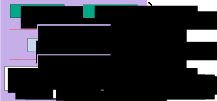
\includegraphics[scale=0.6]{Figures/arquitectura-controlador.pdf}
	\caption{Arquitectura de un controlador \textit{SDN} tradicional.}
	\label{fig:arquitectura_sdn}
  \end{figure}

%----------------------------------------------------------------------------------------
%	SECTION 3
%----------------------------------------------------------------------------------------
\section{Gestión de la Red} \label{sec:gestionred}
En la actualidad se puede encontrar una gran variedad de redes, desde pequeñas redes domésticas de intranet hasta redes empresariales o de proveedores de servicios. Cada una de estas redes tienen diversos requerimientos de gestión.  Las pequeñas redes domésticas, que consisten en unos pocos dispositivos conectados, requieren una sobrecarga de administración baja, y con frecuencia, pueden gestionarse manualmente de forma eficiente. No así las redes más grandes, que podrían contener cientos dispositivos conectados requiriendo un enfoque más sistemático para hacer frente a las complejidades que surgen debido al tamaño de la red. A medida que la red crece en estructura y complejidad, se hace evidente la necesidad de una solución eficiente para la gestión de la misma \parencite{gestionderedes}.

\subsection{Protocolos de Gestión}
Existen múltiples formas de llevar a cabo la administración de la configuración en los diversos dispositivos que conforman la red. En esta sección, se analizarán dos alternativas: \textit{CLI} y \textit{SNMP}.

\subsubsection{\textit{Command Line Interface}}

\textit{CLI} es el enfoque más común en el ámbito de gestión de la configuración, adoptado por múltiples empresas. Consiste en un método para comunicarse con las aplicaciones que la subyacen, a través de una interfaz de usuario simple basada en texto. De esta forma, permite que el administrador pueda ingresar instrucciones en una línea de comandos a través de una terminal y recibir las respuestas en la misma. La aplicación subyacente es la encargada de procesar la instrucción y devolver alguna respuesta al usuario. Generalmente, las respuestas están orientadas a que resulten fácil de entender para las personas, sin embargo, no se encuentran orientadas a las API’s, ya que no existe un formato o un estándar de cómo representar dichas respuestas. Además, las implementaciones internas podrían ser diferentes entre los distintos dispositivos, incluso entre dispositivos del mismo fabricante, de modo que, tanto los comandos como las respuestas podrían variar significativamente entre los equipos.
\\

Un ejemplo de una operación en \textit{CLI} puede verse en la figura \ref{lstlisting:cli}. La primer línea ingresada, hace referencia a un acceso al modo de configuración de un dispositivo cualquiera. En la segunda, se agrega una entrada estática a la tabla de ruteo y en la tercera se abandona el modo de configuración.

\begin{lstlisting}[language=SHELXL, caption=Interacción tipica con un dispositivo mediante \textit{CLI}., label=lstlisting:cli]
	> configure terminal
	#> ip route 192.0.2.0/8 ethernet 1/2 192.0.2.4
	#> !
\end{lstlisting}


  Este enfoque presenta una serie desventajas \parencite{clilimitacion}. En primer lugar, la implementación de las aplicaciones subyacentes a la \textit{CLI} no están estandarizadas, por lo que las operaciones varían drásticamente entre dispositivos de diferentes fabricantes e incluso en implementaciones \textit{CLI} del mismo fabricante. A su vez, los fabricantes podrían brindar una actualización de software del dispositivo, donde los comandos \textit{CLI} de la versión anterior se vean modificados o eliminados, lo que no solo se traduce a problemas para el administrador de red, sino también para las \textit{API’s} que hagan uso de la \textit{CLI}. 
  \\

  En segundo lugar, realizar un cambio en el estado de un dispositivo podría requerir múltiples transacciones, y en el caso de que alguna de estas falle, el dispositivo podría quedar en un estado inconsistente. Por ejemplo, en la figura \ref{lstlisting:cli} se observó que para realizar una operación sencilla como agregar una entrada a la tabla de ruteo, implicó el uso de al menos tres comandos. De forma similar, podrían existir operaciones que requieran de transacciones con una mayor cantidad de instrucciones. \textit{CLI} no define de forma estándar una solución para deshacer los cambios aplicados en el dispositivo.

  \subsubsection{\textit{Simple Network Management Protocol}}
  \textit{SNMP} es un protocolo de monitoreo y administración de red, estandarizado por primera vez en 1988 por la \textit{IETF} \parencite{snmprfc}. Su funcionamiento se basa en una arquitectura cliente-servidor, donde los mensajes se intercambian a través del protocolo de transporte no orientado a la conexión \textit{UDP}. Consiste en una colección de agentes y administradores formando entre ellos una red, donde se denomina administrador a aquel dispositivo que tiene el rol de ejecutar aplicaciones de administración de red, mientras que los dispositivos que requieran ser administrados se denominan agentes \parencite{snmprfcfunc}.

  Las capacidades para administrar la red en \textit{SNMP}, quedan representadas en lo que se conoce como \textit{MIB}. Una \textit{MIB}, es una base de datos que contiene información jerárquica y estructurada en forma de árbol de todos los parámetros gestionables de la red. 
  Dicha base de datos se debe cargar en el administrador \textit{SNMP}, para ello cada agente \textit{SNMP} expone al administrador \textit{SNMP} una serie de módulos \textit{MIB}. Con esta información el administrador podría alterar dinámicamente la configuración del agente. 
  \\

  El uso de \textit{SNMP} como monitoreo es una práctica común desde su publicación, sin embargo, se desalentó su uso en áreas de gestión de configuración por las siguientes razones \parencite{snmplimitacion}: 

  \begin{itemize}
	\item Problemas inherentes al protocolo de transporte \textit{UDP}, donde los mensajes pueden perderse o llegar desordenados, así como también la falta de mecanismos de seguridad para los mismos jugaron un papel importante para reemplazar \textit{SNMP} por otros protocolos de administración de red.
	\item No existe una estandarización de los módulos \textit{MIB} para configurar las funciones de red. El trabajo de descubrir correctamente los módulos \textit{MIB} para cada dispositivo es tarea del usuario, lo que resulta compleja y no eficiente.
\end{itemize}

La figura \ref{fig:snmpfig} muestra las operaciones más comunes de \textit{SNMP}.

\begin{figure}[htbp]
	\centering
	\includegraphics[scale=0.8]{Figures/snmp_ejemplo.pdf}
	\caption{Operaciones tipicas en \textit{SNMP}.}
	\label{fig:snmpfig}
  \end{figure}

\subsubsection{Otras alternativas}
Algunos enfoques para la gestión de la red pueden incluir soluciones basadas en páginas web, que permiten al administrador modificar las configuraciones en el dispositivo de forma gráfica y más amigable, pero generalmente resultan más limitadas que las \textit{CLI}. 
Además, algunos dispositivos pueden brindar soluciones propietarias para la gestión de la configuración, sin embargo, estas soluciones suelen ser muy específicas a un dispositivo o una familia de dispositivos, y rara vez suelen ser compatibles entre sí. Estos últimos también representan una carga para los administradores, donde cada solución requiere que el administrador aprenda otra manera de configurar las funcionalidades de la red.  

\subsection{\textit{NETCONF}}
Esta sección repasa brevemente los conceptos y características principales que ofrece el protocolo \textit{NETCONF}. Además, aspectos de seguridad, transporte y control de acceso del protocolo se discuten en detalle. 

\subsubsection{Definición}
\textit{NETCONF} fue estandarizado por la \textit{IETF} por primera vez en el 2006, en el \textit{RFC 4741} \parencite{netconfrfc}. Actualmente está siendo adoptado por los principales proveedores de dispositivos de red y ha ganado el apoyo de la industria. Según detalla Carl Moberg \parencite{netconfusos}, podemos encontrar que fabricantes como Juniper, Huawei, Cisco, entre otros, brindan soporte desde hace tiempo del protocolo \textit{NETCONF}. 
\\

La \textit{IETF} definde a \textit{NETCONF} como un protocolo estándar para Instalar, manipular y borrar configuraciones en un dispositivo \parencite{netconfrfcnuevo}. Permite implementar una \textit{API} formal utilizando el lenguaje de modelado \textit{YANG} para administrar y monitorear las funcionalidades de la red. \textit{NETCONF} utiliza el paradigma de las \textit{RPC}, donde construye los mensajes que intercambian información como un flujo con codificación \textit{XML}. Funciona con una arquitectura cliente-servidor, donde los mensajes son transportados utilizando algún protocolo orientado a la conexión. El \textit{RFC 6241}, en la sección 1.2, menciona una partición conceptual del protocolo en cuatro capas, dicha partición se refleja en la figura \ref{fig:netconf}. 
\\

A continuación, se explica qué función cumple cada una de estas capas.

\begin{itemize}
	\item \textbf{Capa de transporte seguro:} provee mecanismos de comunicación entre cliente y servidor.  
	\item \textbf{Capa de mensajes:} encargada de la codificación y partición de los mensajes.  
	\item \textbf{Capa de operación:} define las operaciones admitidas por el protocolo.
	\item \textbf{Capa de contenido:} relaciona la representación y el modelado de los datos en el protocolo.    
\end{itemize}

\begin{figure}[htbp]
	\centering
	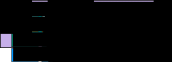
\includegraphics[scale=0.7]{Figures/stack-netconf.pdf}
	\caption{Separación conceptual del protocolo \textit{NETCONF}.}
	\label{fig:netconf}
  \end{figure}


  Las características que destacan a \textit{NETCONF} como protocolo de administración de red son \parencite{netconfpros}:

  \begin{itemize}
	\item Capacidad de restauración de los datos y \textit{backup} de la configuración.
	\item De uso fácil, presentando la información de forma estructurada con una codificación entendible para las personas y las \textit{API’s}.
	\item Implementa mecanismos de control de errores mediante validación de sintaxis y semántica.
	\item Separación clara de los datos de configuración y los datos de estado.
	\item Posibilidad de gestionar la configuración en un dispositivo de manera reactiva mediante notificaciones del mismo.
\end{itemize}

\textit{NETCONF} separa los datos de configuración de los datos de estado de un dispositivo. Según lo detallado en la sección 1.1. y 1.4 del \textit{RFC 6242}, se define a cada uno como:

\begin{itemize}
	\item \textbf{Datos de configuración:} información que se puede leer o escribir y que se utiliza para llevar al dispositivo de un estado inicial a un estado deseado. Un ejemplo es la velocidad del ventilador del cpu del dispositivo.  
	\item \textbf{Datos de estado:} representa información de sólo lectura y estadísticas brindadas por el dispositivo. Por ejemplo, la temperatura del cpu del equipo.   
\end{itemize}

\subsubsection{Conceptos del Protocolo}
Como se mencionó anteriormente, \textit{NETCONF} define un protocolo de administración de red con arquitectura cliente-servidor, donde el cliente en este caso es el sistema de administración de la red o el administrador del sistema, mientras que el dispositivo que contiene una o más funciones de red que deben ser administradas, actúa de servidor. El cliente y el servidor inician la sesión de protocolos mediante un primer mensaje que da lugar al intercambio de capacidades o \textit{capabilities}, donde se definen qué operaciones estarán disponibles para su uso. Este primer mensaje recibe el nombre de \textit{HELLO} \parencite{netconfrfcnuevo}. La figura \ref{fig:netconf_comunicacion} ejemplifica la arquitectura presentada por el protocolo.

\begin{figure}[htbp]
	\centering
	
\includegraphics[scale=0.77]{Figures/netconf-cliente-servidor.pdf}
	\caption{Arquitectura cliente-servidor en el protocolo \textit{NETCONF}.}
	\label{fig:netconf_comunicacion}
  \end{figure}

  \subsubsection{Capacidades}
  El protocolo \textit{NETCONF} está diseñado para ser altamente extensible y, con este fin, es compatible con el intercambio inicial de capacidades entre cliente y servidor \parencite{netconfrfcnuevo}. Este intercambio de información permite al cliente ajustar sus comportamientos basándose en las funcionalidades que admite el servidor. Cada capacidad establecida por el protocolo recibe un nombre asignado por la \textit{IANA}. Además, también se incluye el intercambio de los modelos \textit{YANG} que tiene implementado el servidor, lo cual es necesario no solo para que el cliente pueda aprender de los mismos, sino también para reconocer las diferentes revisiones implementadas en el servidor. 
  \\
  
  La utilidad de esta característica reside en que, a través del intercambio de las capacidades entre el cliente y el servidor, el protocolo define cuáles serán las operaciones admitidas desde el inicio de la sesión, evitando así el ingreso de comandos de configuración incorrectos o no soportados. 


  \subsubsection{Sesión orientada a la conexión}
  La sección dos del \textit{RFC 6242}, referida a protocolos de transporte, detalla que \textit{NETCONF} no esta vinculado a ningún protocolo de transporte específico. El requisito necesario de \textit{NETCONF} para el protocolo de transporte subyacente es que el mismo sea orientado a la conexión. 
  \\

  Esta es una de las principales ventajas frente a \textit{SNMP}, donde los mensajes en este último eran transportados a través del protocolo no orientado a la conexión, \textit{UDP}. Además, el hecho de que \textit{NETCONF} no especifique el uso de un único protocolo de transporte orientado a la conexión, se traduce a una mayor flexibilidad y personalización para el administrador, pudiendo optar por aquella que mejor se ajuste a las necesidades de los equipos involucrados.


  \subsubsection{Sesión orientada a la autenticación}
  El protocolo \textit{NETCONF} es orientado a la sesión con autenticación, utilizando una arquitectura cliente-servidor donde el servidor escucha un puerto asignado para recibir las conexiones con los clientes. 

  Según la sección dos del \textit{RFC 6242} referida a seguridad, el protocolo mínimamente debe ofrecer autenticación, confidencialidad e integridad. Cualquier mensaje \textit{NETCONF}, incluido el mensaje \textit{HELLO}, se envian unicamente si el cliente y servidor se han autenticado de forma correcta. No se especifica un protocolo en particular, pudiendo utilizarse alguno de los múltiples protocolos de transporte seguros existentes en la actualidad como \textit{TLS}, \textit{SSH}, \textit{BEEP}, etc. Cualquier implementación de \textit{NETCONF} debe, al menos, soportar \textit{SSH} como protocolo de transporte seguro.

  Además, según el \textit{RFC 6536} relacionado al control de acceso de usuarios, \textit{NETCONF} admite una jerarquía de niveles de usuarios. Por ejemplo, tener dos grupos de usuarios donde uno tenga permisos de configuración más limitados que el otro.

  \subsubsection{Bases de datos}
  \textit{NETCONF} define en la sección cinco del \textit{RFC 6242}, la existencia de uno o más \textit{datastores}, los cuales cumplen el papel de una base de datos conceptual que puede ser utilizada para almacenar y acceder tanto a los datos de configuración como a los datos de estado. El protocolo especifica y define tres tipos de base de datos: \textit{running}, \textit{startup} y \textit{candidate}, de las cuales únicamente es obligatorio que se implemente la primera. Si la implementación admite otras bases de datos, como por ejemplo \textit{startup} o \textit{candidate}, el servidor informará al cliente esta capacidad en el mensaje \textit{HELLO}. Cada operación en \textit{NETCONF} debe especificar la base de datos a la cual se realizará la consulta o modificación.
  \\

  A continuación, se detalla cada uno de los almacenes de datos mencionadas.
\begin{itemize}
	\item \textbf{\textit{startup}:} según lo especificado en la sección 8.7 del \textit{RFC 6242}, dicha base de datos se utiliza para almacenar de forma persistente la información de configuración del dispositivo. El contenido de esta es copiado de manera automática a la base de datos conocida como \textit{running} en el inicio del servidor \textit{NETCONF}. De esta forma, el protocolo brinda una herramienta al dispositivo para poder aplicar una configuración dado al inicio del equipo. 
	\item \textbf{\textit{running}:} refleja la configuración actualmente en uso por el dispositivo. Es la única base de datos conceptual que admite la presencia tanto de datos de estado como datos de configuración. A alto nivel, esta base de datos diferencia del estado de \textit{startup}, puesto que no es una configuración que será aplicada al inicio sino que refleja la configuración actual del dispositivo.
	\item \textbf{\textit{candidate}:} se encuentra definido en la sección 8.3 del \textit{RFC 6242}. Puede ser utilizado para realizar cambios que no se van a aplicar al dispositivo de forma directa, sino que lo harán una vez se realice un \textit{commit} sobre dicha base de datos. De esta forma, el contenido de \textit{candidate} es copiado a \textit{running}. Si de lo contrario se desea descartar los cambios realizados en este \textit{datastore}, la operación \textit{discard-changes} copia el contenido de \textit{running} a \textit{candidate}. En esta base de datos conceptual únicamente se admiten datos de configuración. En otras palabras, la utilidad de esta base de datos reside en que permite brindar al administrador un entorno de pruebas, donde se podría aplicar una configuración temporal en el equipo, con capacidad de volver a la configuración anterior en caso de fallas.
\end{itemize}


Como se mencionó anteriormente, cualquier implementación de \textit{NETCONF} debe admitir al menos el \textit{datastore running}, esto es necesario ya que los datos de estado (necesarios para monitorear el dispositivo) únicamente se encuentran admitidos en dicho \textit{datastore}.
\\

Por último, se podría hacer una analogía entre la separación de los datos de estado y los datos de configuración con la separación conceptual de dichas bases de datos lógicas. 
En el primer caso, se busca distinguir entre un dato de solo lectura de otro que admite la escritura, mientras que el segundo trata de diferenciar entre un conjunto de estados bien definidos que puede alcanzar el dispositivo. Por ejemplo, distinguir la configuración que va a aplicarse únicamente en el inicio del dispositivo a través del \textit{datastore startup}, de la configuración que podría llevar en un determinado momento a través del \textit{datastore running}.


\subsubsection{Operaciones del protocolo}

Las operaciones en el protocolo \textit{NETCONF} se definen como \textit{RPC} en los modelos \textit{YANG} relevantes. En dichos modelos también se definen los argumentos de entrada y los contenidos de salida para cada operación. Todas las operaciones están codificadas en \textit{XML} dentro de los mensajes \textit{RPC} que son, de hecho, los únicos mensajes que los clientes pueden enviar en las sesiones de \textit{NETCONF} después del intercambio inicial del mensaje \textit{HELLO}. 
\\

Como las operaciones son \textit{RPC}, cada mensaje enviado por los clientes tendrá una respuesta por parte del servidor. Este resultado normalmente contiene \textit{ok} para indicar que la operación resultó según lo esperado, o \textit{error} indicando las razones por la cual falló dicha operación.
\\

El protocolo define en la sección 7 del \textit{RFC 6241} nueve operaciones básicas y necesarias para cualquier implementación del mismo, las cuales se describen a continuación:

\begin{itemize}
	\item \textbf{\textit{get}:} utilizado para consultar tanto datos de configuración como datos de estado al servidor \textit{NETCONF}.
	\item \textbf{\textit{get-config}:} operación que devuelve los datos de configuración del dispositivo. Puede incluir filtros para limitar la información enviada por parte del servidor.
	\item \textbf{\textit{edit-config}:} definida para crear, actualizar o borrar datos de configuración en el servidor. Únicamente se admite esta operación en las bases de datos \textit{running} o \textit{candidate}.
	\item \textbf{\textit{copy-config}:} crea o reemplaza completamente el contenido de una base de datos por otra. El caso de uso más común de esta operación es para copiar el contenido del \textit{datastore running} al \textit{datastore startup}. 
	\item \textbf{\textit{delete-config}:} Elimina completamente el contenido de un \textit{datastore} determinado. No se admite esta operación para la base de datos \textit{running}.
	\item \textbf{\textit{lock}:} permite al cliente bloquear la configuración completa de un \textit{datastore} específico en un dispositivo. Tales bloqueos son destinados a ser de corta duración, de esta forma un cliente puede realizar un cambio sin temor a la interacción con otros clientes de \textit{NETCONF}. Además, como el protocolo es orientado a la sesión, todos los recursos tomados por la misma tales como los datastores, deben ser liberados en el momento de la finalización o cierre de la sesión.
	\item \textbf{\textit{unlock}:} permite a la sesión liberar el recurso tomado por la operación lock.
	\item \textbf{\textit{close-session}:} utilizada para finalizar la sesión entre cliente y servidor \textit{NETCONF}. Cualquiera de las operaciones mencionadas en esta sección, quedan inhabilitadas una vez finalizada la sesión.
	\item \textbf{\textit{kill-session}:} permite al administrador de red finalizar alguna sesión inactiva que tiene recursos tomados. 
\end{itemize}

Además de estas nueve operaciones descritas por el protocolo, pueden proporcionarse operaciones adicionales basado en las capacidades anunciadas por el dispositivo, como por ejemplo operaciones \textit{RPC} definidas en los módulos \textit{YANG}.
\\

También, \textit{NETCONF} admite operaciones con capacidades más avanzadas. No es obligatorio que las diferentes implementaciones del mismo soporten las siguientes características, más bien, de hacerlo deben ser expuestas como capacidades admitidas en el mensaje \textit{HELLO}. Dichas operaciones se describen a continuación:
\begin{itemize}
	\item \textbf{\textit{commit}:} operación utilizada para copiar atómicamente el contenido del \textit{datastore candidate} al \textit{datastore running}. Además, puede incluirse la operación \textit{confirmed-commit}, esta última funciona como un \textit{backup} de la configuración previa al \textit{commit}, la cual se restablece al cabo de un \textit{timeout} si no se recibe la operación \textit{confirmed-commit}. \textit{NETCONF} describe a esta última como una 'confirmación de la confirmación'.
	\item \textbf{\textit{discard-changes}:} revierte una operación que está en espera de confirmación. En otras palabras, se copia el contenido del \textit{datastore running} al \textit{datastore candidate}.
	\item \textbf{\textit{validate}:} consiste en una operación que verifica la correctitud semántica y sintáctica de una configuración antes de aplicar el cambio en el dispositivo. 
\end{itemize}


La tabla \ref{Tab:netconf_operaciones} resume las diferentes operaciones disponibles en \textit{NETCONF} y a qué \textit{datastore} podría aplicarse cada una de ellas. 
\\

\begin{table}[H]
	\centering
	\begin{tabular}{|c|c|c|}
	\hline
	\textbf{Capacicad}        & \textbf{Operación}                                                                                                       & \textbf{Base de datos afectada}                                                                                                                                     \\ \hline
	\textbf{writable-running} & \begin{tabular}[c]{@{}c@{}}lock\\ edit-config\\ unlock\\ copy-config\end{tabular}                                        & \begin{tabular}[c]{@{}c@{}}running\\ running\\ running\\ running -\textgreater startup\end{tabular}                                                                 \\ \hline
	\textbf{candidate}        & \begin{tabular}[c]{@{}c@{}}lock\\ edit-config\\ commit\\ validate\\ unlock\\ copy-config\end{tabular}                    & \begin{tabular}[c]{@{}c@{}}candidate\\ candidate\\ candidate -\textgreater running\\ candidate\\ candidate\\ running -\textgreater startup\end{tabular}             \\ \hline
	\textbf{confirmed-commit} & \begin{tabular}[c]{@{}c@{}}lock\\ edit-config\\ commit\\ confirmed-commit\\ validate\\ unlock\\ copy-config\end{tabular} & \begin{tabular}[c]{@{}c@{}}candidate\\ candidate\\ candidate\\ candidate -\textgreater running\\ candidate\\ candidate\\ running -\textgreater startup\end{tabular} \\ \hline
	\end{tabular}
	\caption{Ejemplo de operaciones disponibles en \textit{NETCONF}}
	\label{Tab:netconf_operaciones}
	\end{table}


  \subsubsection{Notificaciones}

  Si bien \textit{NETCONF} está diseñado principalmente para la administración de la configuración de la red mediante las operaciones expuestas anteriormente, existe una poderosa herramienta de monitoreo implementada en el protocolo llamada notificaciones. La \textit{RFC 5277} define a las mismas como un servicio de entrega de mensajes asíncronas a los clientes mediante suscripción. Esta característica no es obligatoria para las diferentes implementaciones del protocolo. De soportarlo, el servidor deberá comunicar a los clientes dicha característica como una capacidad del servidor en el mensaje \textit{HELLO}.
  \\

  Esta herramienta es similar a las notificaciones en el protocolo \textit{SNMP}, pero tiene la ventaja de que, en \textit{NETCONF}, el cliente puede especificar a qué notificación particular se desea suscribir, lo que permite un monitoreo más flexible. Además, como se mencionó anteriormente, el servidor puede declarar permisos para los diferentes usuarios y sesiones por lo que las notificaciones serán enviadas únicamente a aquellos clientes suscritos y que cumplan con el nivel de acceso requerido por el servidor.
  \\

  La importancia de las notificaciones reside en que los dispositivos de red tienen variables críticas que deben ser monitoreadas, por ejemplo la temperatura del equipo, el estado de los enlaces, la conectividad entre los mismos, etc. Dichas variables críticas reciben el nombre de alarmas. 
  
  De no existir un mecanismo de mensajes asíncronos, el monitoreo de las alarmas de un dispositivo podría implicar una sobrecarga en la red, debido a la cantidad de consultas periódicas que existirían sobre los dispositivos. 


  De esta forma, las notificaciones que define el protocolo \textit{NETCONF} no solo implica un monitoreo eficiente mediante mensajes asíncronos, sino que permite al protocolo poder tomar medidas de forma reactiva a las diferentes alarmas que se presenten. Por ejemplo, se podría configurar al cliente \textit{NETCONF} para que, de recibir una alarma de exceso de temperatura en el equipo, configure de forma automática una velocidad mayor en el ventilador del mismo. 
  \\

  Para finalizar, la figura \ref{fig:netconf_ejemplo} refleja una interacción típica entre cliente y servidor donde se observa el intercambio de capacidades en los mensajes \textit{HELLO}, el uso de diferentes operaciones con respuestas \textit{RPC} y las notificaciones.

  \begin{figure}[!h]
	\centering
	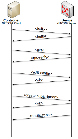
\includegraphics[scale=0.8]{Figures/netconf_ejemplo.pdf}
	\caption{Ejemplo de comunicación entre cliente y servidor NETCONF.}
	\label{fig:netconf_ejemplo}
  \end{figure}

  \subsection{Lenguaje de Modelado \textit{YANG}}
  Como se mencionó anteriormente, \textit{NETCONF} utiliza \textit{YANG} para modelar los datos de estado, los datos de configuración, las \textit{RPC} y las notificaciones. \textit{Yet Another Next Generation} es un lenguaje de modelado de datos desarrollado y estandarizado en la \textit{RFC 6020} por la \textit{IETF} en el año 2010 \parencite{yangrfc}. Si bien existen en la actualidad lenguajes de modelado como \textit{XML Schema}, \textit{SMI}, \textit{UML}, entre otros, la ventaja que presenta \textit{YANG} frente a los demás es que es un lenguaje de modelado específico para gestión de la configuración de red.

  \subsubsection{Conceptos del Lenguaje}
  \textit{YANG} define, en la sección 4.1 de la \textit{RFC 6020}, las funcionalidades de la red separando los datos de estado de los datos de configuración y presentando la información como una estructura de árbol jerárquica. Consiste en una serie de declaraciones y tipos que pueden ser usadas para definir los datos que se quieren modelar. Estas definiciones son contenidas en un módulo y describen qué tipo de datos admite una variable. A su vez, un módulo puede heredar definiciones de otro módulo.

  \subsubsection{Módulos y submódulos}
  Definen una estructura para el modelado de datos. Tienen un diseño predefinido que se debe seguir. Este diseño comienza con un encabezado, siguiendo de las declaraciones que contenga el módulo y por último las revisiones y comentarios respecto al mismo. 
  \\

  Se define el nombre del módulo, un prefijo para identificarlo, las dependencias, información de contacto al autor, descripción y revisiones. La declaración \textit{'include'} permite referenciar material que se describe en un submódulo, mientras que la declaración \textit{'import'} permite referenciar material que se encuentra descrito en un módulo externo. La estructura básica de un módulo puede verse en la figura \ref{fig:estructura_modulo}.

  \begin{figure}[htbp]
	\centering
	\includegraphics[scale=0.4]{Figures/estructura_modulo.pdf}
	\caption{Estructura de un módulo \textit{YANG}.}
	\label{fig:estructura_modulo}
  \end{figure}

  \subsubsection{Declaraciones y Definiciones de Datos}
  A continuación, se describen algunas sentencias que podría contener un módulo \textit{YANG}. Cada sentencia contiene la definición del tipo de dato y puede contener además algún valor para ese tipo de dato. Siempre representan a datos de configuración o datos de estado, realizando dicha distinción con la sentencia llamada \textit{'config'}.  

  \begin{itemize}
	\item \textbf{\textit{leaf}:} contiene un dato simple como un entero o un \textit{string}. Admite exactamente un valor para un tipo de dato particular y opcionalmente puede incluir una descripción. 
	\item \textbf{\textit{leaf-list}:} describe una secuencia de datos tipo \textit{leaf}. Cada \textit{leaf} admitirá un solo valor para el tipo de dato que especifique el \textit{leaf-list}.
	\item \textbf{\textit{container}:} es utilizado para agrupar datos lógicamente relacionados. Un \textit{container} no admite un valor, pero sí admite cualquier número de tipos de datos como \textit{leaf}, \textit{leaf-list}, \textit{container} o \textit{list}.
	\item \textbf{\textit{list}:} define una secuencia de tipo de datos donde cada tipo de dato es única, identificado por la sentencia \textit{key}. Puede contener múltiples identificadores \textit{key} y cualquier cantidad de tipo de datos \textit{leaf}, \textit{leaf-list}, \textit{container}, etc.
	\item \textbf{\textit{choices - cases}:} no describen algún tipo de dato, más bien ofrecen ramificaciones condicionales en la estructura del módulo. La sentencia \textit{choice} es una condición que asegura que, como máximo, se cumplira una de las declaraciones dadas por case.
\end{itemize}

Las declaraciones y sentencias descritas anteriormente pueden ser utilizadas en conjunto para poder formar una estructura de datos tipo árbol más compleja.
Además, \textit{YANG} admite la reutilización de sentencias mediante las declaraciones \textit{include} e \textit{import} reduciendo así los posibles errores en el modelado de datos.

\subsubsection{Identificador de instancia }
Cada dato en \textit{YANG}, así como el propio módulo, tiene un identificador único de instancia que se puede utilizar para referirse a él. Los identificadores se denominan \textit{namespace}, y admiten un prefijo para poder acortar el nombre. 
\\

Por ejemplo, Bjorklund \parencite{yangsystem}, definió un módulo \textit{YANG} para la administración de interfaces. Dicho modelo tiene una estructura de datos de tres niveles para una interfaz básica. En el nivel superior del modelo se encuentra definido el \textit{container} llamado \textit{'interface'}, seguido de la \textit{list 'interface'} que contiene múltiples instancias de una interfaz, identificada por la \textit{key 'name'}. Además, cada interfaz tiene una \textit{leaf 'enabled'} que describe el estado de la misma. Un ejemplo de identificador para una instancia de \textit{'interface'} llamada \textit{'eth0'} puede verse en la figura \ref{fig:interfaceyang}.

\begin{figure}[htbp]
	\centering
	\includegraphics[scale=0.9]{Figures/interface-yang.pdf}
	\caption{Ejemplo de identificador de instancia en \textit{YANG}.}
	\label{fig:interfaceyang}
  \end{figure}

  \subsubsection{Funcionalidades}
  \textit{YANG} ofrece características especiales que lo distinguen de un documento \textit{JSON}, permitiéndole describir de forma eficiente las funcionalidades de la red. Estas características incluyen la validación de modelos, una forma estandarizada de extender a los módulos y compatibilidad entre las diferentes revisiones de los mismos. En esta sección, se analizaron las principales funcionalidades ofrecidas por \textit{YANG}.

  \begin{itemize}
	\item \textbf{Validación:} una de las características más importantes de \textit{YANG} es la posibilidad de validar automáticamente todos los datos descritos en el modelo. Resulta importante ya que la validación de los datos es una tarea difícil. Dicha afirmación está respaldada por el hecho de que introducir datos erróneos y tomarlos como válidos, está catalogada como la principal amenaza de seguridad según \textit{OWASP} \parencite{owasp}, organización sin ánimo de lucro a nivel mundial dedicada a mejorar la seguridad de las aplicaciones y del software en general. Cada dato introducido en el modelo \textit{YANG} puede ser validado semánticamente y sintácticamente. La validación de sintaxis es automática y garantiza que el dato contenga una secuencia de bytes válido, puesto que cada dato en el modelo tiene asociado un \textit{type} (string, int, uint, etc). Por otra parte, la validación semántica resulta más compleja y puede ser usada para describir dependencias entre datos. \textit{YANG} también admite sentencias como \textit{'when'} o \textit{'must'} que pueden ser usadas para evaluar condicionalmente un dato.  
	\item \textbf{Compatibilidad:} cada módulo admite la indicación de una revisión, esto permite a \textit{YANG} distinguir las versiones soportadas y adaptarse a la situación cuando la misma no es soportada. También, se describen reglas de actualización en los módulos que deben respetarse para mantener compatibilidad entre los modelos de datos anteriores. Por ejemplo, cualquier cambio en un módulo debe indicar una revisión en la cabecera, tanto el nombre del mismo como el namespace debe mantenerse, como así también las definiciones de datos obsoletas, lo que permite compatibilidad con modelos de datos anteriores. Esta característica permite a los módulos evolucionar con el paso del tiempo, sin romper aplicaciones existentes con versiones anteriores.
	\item \textbf{Extensión:} permite extender las funcionalidades de los módulos con nuevas definiciones de datos. Existen muchas razones por las cuales utilizar la extensión en \textit{YANG}, como por ejemplo, desarrollar un nuevo módulo a partir de uno existente o con el fin de reducir errores reutilizando un módulo funcional. Una ventaja importante que tiene utilizar la extensión, es que al agregar nueva información en un módulo, se mantiene compatibilidad con el heredado.
\end{itemize}

\subsection{Redes Ópticas de Transporte}
La explosión del tráfico digital provocado por los nuevos enfoques como \textit{Big Data} o el \textit{Streaming}, y los requerimientos de los usuarios donde existe un constante crecimiento de aplicaciones con alta demanda de ancho de banda, requieren de una nueva tecnología de transporte que pueda ocuparse de los patrones de tráfico y los contenidos de datos modernos. Para ello, se han realizados numerosos avances en los últimos años referente al plano de control y el plano de datos de las redes ópticas \parencite{redesopticas}, surgiendo protocolos como SONET o OTN. En esta sección, se analiza las redes ópticas, utilizadas para el transporte de los datos como así también los dispositivos que funcionan sobre dichas redes. 
\\

Una red de transporte óptica, es un tipo de red de comunicaciones de datos que utiliza la luz como medio de transporte para la información \parencite{redesopticasdef}. A diferencia de las redes basadas en cobre, los pulsos de luz de una red óptica pueden transportarse a una distancia considerable e incluso regenerarse a través de un dispositivo repetidor óptico. Después de que una señal óptica es recibida en su red de destino, la misma se convierte en una señal eléctrica a través de un receptor óptico, para luego ser enviado al nodo de la capa de paquetes. 
\\

Un sistema de comunicaciones ópticas puede incluir diversos dispositivos, como ser:

\begin{itemize}
	\item \textbf{Amplificadores ópticos}. 
	\item \textbf{\textit{Switches} ópticos,} encargados de conmutar de un canal a otro.
	\item \textbf{Divisores de luz,} cuya tarea comprende dividir la señal en diferentes caminos de fibra óptica.
	\item \textbf{Fibra óptica,} que cumple de medio de transporte de la información entre los diferentes equipos.
	\item \textbf{\textit{Transponders} y \textit{Muxponders},} encargados de enviar y recibir las señales ópticas por las fibras. Generalmente son caracterizados por el ancho de banda que pueden transportar y la distancia que puede alcanzar la transmisión.
\end{itemize}

\subsubsection{\textit{Transponders} y \textit{Muxponders}}
El \textit{transponder}, es un dispositivo que recibe múltiples señales ópticas a través de sus puertos clientes, dichas señales ópticas pueden tratarse de servicios diferentes como por ejemplo, \textit{Ethernet}, \textit{SONET}, \textit{OTN}, entre otros. Luego, transforma estas señales en flujos de datos eléctricos, las procesa y regenera las mismas para nuevamente convertirlas en señales ópticas compatibles con el estándar \textit{ITU}. De esta forma, realiza la función de recepción, amplificación y reemisión de una señal óptica en un proceso que comúnmente se denomina \textit{optical electrical optical} (OEO) \parencite{transpondermux}.
\\

La figura \ref{fig:transponder} ejemplifica el proceso \textit{OEO} típico de un \textit{transponder}.

\begin{figure}[H]
	\centering
	\includegraphics[scale=0.9]{Figures/transponder.pdf}
	\caption{Funcionamiento básico de un \textit{transponder}.}
	\label{fig:transponder}
  \end{figure}

  Por otra parte, los \textit{muxponders} realizan una función similar a los \textit{transponders}. También incluyen el proceso \textit{OEO}, con la diferencia de que combinan múltiples servicios en una sola longitud de onda que luego se multiplexan en la misma fibra \parencite{transpondermux}. Por lo tanto, en lugar de asignar a cada servicio una longitud de onda dedicada, permite que varios servicios diferentes compartan la misma longitud de onda. Estos dispositivos maximizan la utilización de la fibra y ofrecen soluciones de bajo costo para empresas y transportistas. La figura \ref{fig:muxponder} muestra el comportamiento de un \textit{muxponder}.

  \begin{figure}[htbp]
	\centering
	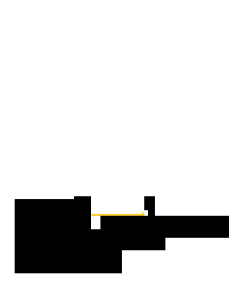
\includegraphics[scale=0.9]{Figures/muxponder.pdf}
	\caption{Funcionamiento básico de un \textit{muxponder}.}
	\label{fig:muxponder}
  \end{figure}

  \subsubsection{Aplicaciones}
  Resulta importante ahora separar la red en dos capas diferentes: la capa de paquetes o de \textit{IP/MPLS}, y la capa óptica o de transporte \parencite{capasredess}. La figura \ref{fig:capasredes} muestra dicha separación.  Los dispositivos mencionados anteriormente se utilizan en la capa de transporte mientras que los \textit{routers} y \textit{switches} convencionales se encuentran en la capa \textit{IP/MPLS}.
  \\

La función que tienen los \textit{muxponders} es la de proveer una conexión lógica entre los diferentes \textit{routers}, quienes podrían estar separados por enormes distancias donde los protocolos como \textit{Ethernet} no proveen un buen servicio de transporte. 
\\

De esta forma, los dispositivos de la capa \textit{IP/MPLS} tienen conocimiento de sus vecinos pero no de la forma en la que se encuentran conectados ni de cómo se está realizando dicha comunicación, mientras que los equipos de la capa óptica esencialmente emparejan a los dispositivos de la capa \textit{IP/MPLS}, pero sin tener conocimiento sobre los diferentes servicios que se prestan. 
\\

\begin{figure}[htbp]
	\centering
	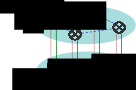
\includegraphics[scale=0.7]{Figures/capasredes.pdf}
	\caption{Separación de la red en capa de paquetes y capa de transporte.}
	\label{fig:capasredes}
  \end{figure}
% % Chapter Template 
% cSpell: words Mininet prototipado parencite enrutamiento includegraphics veth  mininetonf cellcolor Nicira vswitchd interconectar multicapa datapath ovsflow resizebox flowtable netlink OVSDB dpctl ofctl vsctl rowcolor mininetovs
 
\chapter{Análisis de las tecnologías} % Main chapter title

\label{Chapter3} % Change X to a consecutive number; for referencing this chapter elsewhere, use \ref{ChapterX}

Teniendo en cuenta los conceptos revisados en el capítulo anterior, en este se estudiarán las herramientas que permitirán la realización del proyecto. 

En la primera sección, se realizará un análisis del dispositivo utilizado, un \textit{muxponder} óptico coherente de 40Gb desarrollado por la institución donde se realizó el proyecto.
Luego, en la segunda sección se examinarán las herramientas de \textit{software} involucradas. La misma se encuentra dividida en dos partes; la primera detalla el funcionamiento del controlador \textit{SDN} utilizado, \textit{ONOS}; la segunda refiere al estudio de dos agentes \textit{NETCONF}: Sysrepo y Yuma123.


%----------------------------------------------------------------------------------------
%	SECTION 1
%----------------------------------------------------------------------------------------

\section{Herramientas de \textit{Hardware}}

Para cumplir con el objetivo del proyecto, será de importancia conocer las bondades y las limitaciones del equipo con el que se cuenta. Así, esta sección comprende el estudio de uno de los dispositivos mencionados en el capítulo anterior, un \textit{muxponder}. Concretamente, se analizarán aspectos técnicos relacionados tanto al hardware como al \textit{software} de un \textit{muxponder} de 40Gb. El interés de este análisis resulta en que es en este dispositivo en donde se integrará el protocolo de gestión \textit{NETCONF}.

\subsection{\textit{Muxponder} 40Gb}

El equipo en cuestión, es capaz de realizar una transmisión óptica de 40Gb/s sobre una señal de línea \textit{OTU3}. La misma es lograda cumpliendo el estándar \textit{ITU-T G.709} \parencite{itu7}, utilizando una modulación coherente \textit{DP-QPSK} o \textit{DP-DQPSK}.

Cuenta con cuatro clientes ópticos asíncr\textit{onos} totalmente independientes de 10Gb/s cada uno, a través de módulos ópticos  \textit{XFP} removibles. Las longitudes de ondas soportadas para los clientes son 850/1310/1550 nm y admite los tipos de cliente \textit{10Gb Ethernet LAN/WAN, OTU2} y \textit{OTU2e}.

Además, incorpora el mecanismo de corrección de errores \textit{FEC} para todas las señales, tanto para clientes como para línea. Mediante el mismo, el \textit{muxponder} es capaz de realizar correcciones sin necesidad de retransmitir la información.
\\

En términos de potencia, alcanza típicamente los 93 Watts. También, incorpora un amplificador óptico, el cual le permite alcanzar una distancia de hasta 2000Km. Si no se utiliza dicho amplificador, puede alcanzar una distancia de hasta 65Km.
\\

Las interfaces de conexión soportadas para realizar configuración y monitoreo en el dispositivo son: 
\begin{itemize}
	\item 2 puertos \textit{Ethernet} 10/100/1000 Mb/s.
	\item 1 puerto serial \textit{RS232}.
	\item 1 puerto \textit{USB} 2.0.
\end{itemize}

En la figura \ref{fig:mux40} se puede observar en el panel frontal del equipo y las diferentes interfaces mencionadas anteriormente.


\begin{figure}[H]
	\centering
	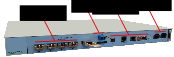
\includegraphics[scale=0.7]{Figures/mux40.pdf}
	\caption{Vista del panel frontal del \textit{muxponder} de 40Gb utilizado.}
	\label{fig:mux40}
  \end{figure}

El \textit{muxponder} de 40Gb integra un total de 128Mb de memoria \textit{RAM} y [[[[]]]] de almacenamiento, con capacidad de extender esta última mediante una tarjeta \textit{SD}. Además, cuenta con un sistema operativo Linux \textit{“Buildroot”}, el cual ocupa gran parte de estos recursos mencionados, dejando libre para las aplicaciones de usuario un total de 100Mb de \textit{RAM} y [[[[]]]] de almacenamiento.

El hecho de que presente dicho sistema operativo resulta en una ventaja por varios motivos, en primer lugar porque el mismo es un entorno conocido por el alumno, donde además podrán ejecutarse en él la mayoría de las aplicaciones \textit{UNIX} típicas. En segundo lugar, el sistema operativo integra librerías y herramientas que facilitaran el desarrollo del proyecto, como por ejemplo la librería \textit{SSH}, necesaria por el protocolo \textit{NETCONF}.
\\

Por último, el procesador que incorpora es un \textit{NIOS II} de primera generación fabricado por \textit{Intel} \parencite{intelaltera}. El mismo funciona a 125 Mhz y se encuentra integrado en una \textit{FPGA}. Es importante destacar que la arquitectura de este procesador no es la arquitectura típica de una máquina de propósito general (por ejemplo $x86_64$), por lo tanto, las distintas aplicaciones que se ejecuten en esta plataforma deberán estar compiladas específicamente para la arquitectura \textit{NIOS}. 

Además, debido a los recursos limitados con los que cuenta el equipo, resulta imposible realizar la compilación de las aplicaciones sobre el mismo equipo. Se deberá realizar lo que se conoce como compilación cruzada, que consiste en preparar un sistema huésped (donde generalmente dicho sistema cuenta con mayores recursos y capacidades) para generar todos los binarios y librerías que requiere  el dispositivo objetivo donde finalmente se ejecutarán las aplicaciones.

%----------------------------------------------------------------------------------------
%	SECTION 2
%----------------------------------------------------------------------------------------

\section{Herramientas de \textit{Software}}

Además del estudio del \textit{hardware} utilizado, resulta de interés realizar un análisis de los componentes de \textit{software} que conforman el proyecto. Para ello, la primer parte de esta sección estará dedicada a estudiar el controlador \textit{SDN} empleado, mientras que en la segunda parte se analizarán dos agentes \textit{NETCONF} disponibles de código abierto.

\subsection{Controlador \textit{ONOS}}
Desarrollado por la \textit{ONF} \parencite{onff}, es uno de los controladores abiertos más comunes en la industria, donde destacan miembros como Google, Intel, AT$y$T, Samsung, entre una numerosa lista \parencite{onffmembers}. Está diseñado específicamente para los proveedores de servicios, donde sus principales objetivos son la escalabilidad y el alto rendimiento \parencite{onffwhite}.

Las licencias compatibles con \textit{ONOS} son \textit{Apache} 2.0, \textit{MIT} y \textit{BSD} \parencite{onfflic}. El hecho de que sea un proyecto \textit{open-source}, supone ventajas como ser interoperabilidad, personalización, flexibilidad e independencia del fabricante. 

Antes de detallar cómo funciona y realizar un análisis de su arquitectura, es importante explicar el problema que enfrentan los controladores \textit{SDN} para poder entender las ventajas que supone el mismo. 
\\

Debido al crecimiento del consumo de tráfico en las redes y la demanda del ancho de banda en alza, es necesario para los proveedores de servicio que el rendimiento y la escalabilidad de sus redes no se vean afectadas por estos motivos. De este modo, los controladores \textit{SDN} deben poseer tres atributos claves: escalabilidad, rendimiento y alta disponibilidad \parencite{sdnproblema}.

\begin{itemize}
	\item \textbf{Escalabilidad}: como se explicó en el capítulo anterior, \textit{SDN} introduce una autoridad de control centralizada. La misma, debe ser capaz de escalar de igual forma que las funcionalidades de la red, manteniendo su rendimiento.
	\item \textbf{Alta disponibilidad}: el plano de control que se encuentra centralizado en el controlador, juega ahora un papel crítico. Las diferentes soluciones \textit{SDN} deberán brindar disponibilidad ininterrumpida del controlador.
	\item \textbf{Rendimiento}: el controlador también tiene que ser capaz de proveer mecanismos para adaptarse dinámicamente ante las fluctuaciones en la carga del tráfico y la congestión de la red. 
\end{itemize}

\subsubsection{Arquitectura}
Las características más importantes de la arquitectura presentada por \textit{ONOS} \parencite{onffwhite} se detallan a continuación:

\begin{itemize}
	\item \textbf{Núcleo distribuido}: la solución que propone \textit{ONOS} para proveer escalabilidad, alto rendimiento y disponibilidad se basa en un núcleo distribuido por los diferentes nodos que conforman un \textit{cluster}, lo que implica la posibilidad de soportar enormes cantidades de dispositivos de red. 
	
	La figura \ref{fig:onosdistribuido} ejemplifica dicha distribución. El hecho de agregar esta redundancia implica una mayor disponibilidad del controlador. A su vez, permite realizar un balanceo de carga, lo que implica mayor rendimiento y escalabilidad.


	\item \textbf{Abstracción \textit{Northbound}}: el plano aplicación, explicado en el capítulo anterior, se comunica con \textit{ONOS} a través de una interfaz brindada por el controlador. El mismo, brinda a las aplicaciones gráficos y estadísticas de la red como así también aplicaciones basadas en intents para facilitar el control, administración y configuración de los equipos.
	\item \textbf{Abstracción \textit{Southbound}}: de forma similar, el controlador ofrece una interfaz para comunicarse con el plano de datos. Cabe destacar que si bien \textit{ONOS} basa su funcionamiento en el protocolo \textit{OpenFlow}, también brinda soporte a otros como \textit{NETCONF}, \textit{REST}, \textit{SNMP}, etc, con el fin de mantener compatibilidad con dispositivos más antiguos.
	\item \textbf{Modularidad}: el controlador se encuentra desarrollado en \textit{Java}, obteniendo así una arquitectura modular. De esta forma, se provee a los desarrolladores facilidad para brindar actualizaciones a sus aplicaciones, poder monitorearlas, realizar depuración y mantenimiento.  
\end{itemize}

\begin{figure}[H]
	\centering
	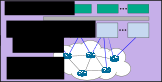
\includegraphics[scale=0.8]{Figures/onosarch.pdf}
	\caption{Arquitectura distribuida de \textit{ONOS}.}
	\label{fig:onosdistribuido}
  \end{figure}

  Para finalizar, se observa en la figura \ref{fig:onosarch} la arquitectura desplegada por ONOS.

  \begin{figure}[H]
	\centering
	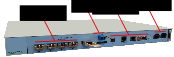
\includegraphics[scale=0.9]{Figures/mux40.pdf}
	\caption{Vista del panel frontal del \textit{muxponder} de 40Gb utilizado.}
	\label{fig:onosarch}
  \end{figure}

  \subsubsection{Interfaz Southbound en ONOS}
  Tal como se explicó anteriormente, el objetivo del proyecto es gestionar la configuración de un \textit{muxponder} de 40Gb a través del protocolo \textit{NETCONF}. Para ello, se procede a explicar con más detalle la interfaz \textit{Southbound} de \textit{ONOS}. La misma, se encuentra dividida en una serie de componentes que se detallan a continuación:

  \begin{itemize}
	\item \textbf{\textit{Providers}}: son aplicaciones independientes que residen en el núcleo de \textit{ONOS}, las mismas pueden activarse o desactivarse dinámicamente en tiempo de ejecución. El propósito principal de esta capa es abstraer al \textit{core} las complejidades de los protocolos, brindando interfaces a las operaciones típicas de los mismos. Un ejemplo de un \textit{provider} en \textit{ONOS} es el llamado \textit{“NetconfAlarmProvider”}, encargado de transformar cada notificación de los dispositivos en una alarma registrada en \textit{ONOS}.
	\item \textbf{\textit{Protocols}}: es la capa de más bajo nivel en la interfaz \textit{Southbound} y es la única que tiene contacto directo con los dispositivos conectados al controlador. Aquí se implementan los diferentes protocolos necesarios para la comunicación como ser \textit{NETCONF}, \textit{REST}, \textit{SNMP}, etc. Comúnmente se utilizan librerías de terceros como \textit{openflowj, snmp4j, thrift}, entre otras.
	\item \textbf{\textit{Drivers}}: al igual que los \textit{providers}, los \textit{drivers} pueden cargarse dinámicamente al núcleo del controlador y proveen mecanismos para comunicarse con los diferentes dispositivos a través de algún protocolo. La diferencia principal con los \textit{providers} es que aquí no se implementan generalidades de los protocolos, sino comportamientos específicos de los dispositivos. Además, sirve de interfaz entre las aplicaciones que se encuentran en la capa \textit{Northbound} y los diferentes equipos de red.  El propósito principal de este subsistema es el de aislar el código específico del dispositivo de tal manera de que el mismo no se extienda por el resto del núcleo de \textit{ONOS}. Dado que tal código será necesario para cualquier futuro previsible, este subsistema proporciona medios para contenerlo y permitir que otros subsistemas interactúen con él a través de abstracciones independientes del protocolo y del dispositivo. Por último, presenta una ventaja para los desarrolladores de hardware dado que al ser un componente modular, permite la herencia de funcionalidades de otros \textit{drivers} con el fin de compartir características con una familia de dispositivos en común.
\end{itemize}

La figura \ref{fig:onosarchsouth} esclarece la participación que tiene cada componente tanto con el \textit{core} como con el dispositivo.

\begin{figure}[H]
	\centering
	
\includegraphics[scale=0.85]{Figures/southboundonos.pdf}
	\caption{Interfaz \textit{Southbound} en \textit{ONOS}.}
	\label{fig:onosarchsouth}
  \end{figure}

  \subsubsection{Justificación de la elección del controlador}

En la actualidad, existe una diversidad de controladores \textit{SDN}, como ser \textit{Ryu} (\textit{Python}), \textit{Floodlight} (\textit{Java}), \textit{POX} (\textit{Python}), e incluso implementaciones propietarias. 

Se destaca \textit{OpenDaylight} (\textit{Java}), un controlador abierto que soporta una gran lista de protocolos y que, según [], junto a \textit{ONOS} es uno de los controladores más utilizados en la industria.

La razón determinante por la cual se optó por \textit{ONOS} como controlador \textit{SDN} radica en que el mismo cuenta con una documentación más clara y organizada. Esto facilitó la curva de aprendizaje de las distintas herramientas, donde se pudo tener una rápida interacción con el controlador dada su facilidad de instalación y puesta en marcha.

Otro motivo reside en que las redes de los proveedores de servicio son complejas y multicapas, donde se requiere una separación clara de la capa de paquetes y de la capa de transporte, tal como se vió en el capítulo anterior. \textit{ONOS}, ha logrado brindar soporte a las redes ópticas según lo demuestra el caso de uso aquí descripto [].

\subsection{Análisis de agentes \textit{NETCONF}}

Con el fin de poder gestionar la configuración del \textit{muxponder} de 40Gb a través de \textit{NETCONF}, se estudiará en esta sección dos implementaciones del protocolo: Sysrepo y Yuma123. 

Las mismas son \textit{open-source}, lo que facilita el estudio y comprensión de los agentes. Finalmente, se justificará la elección de Yuma123 como servidor \textit{NETCONF} para el proyecto.

\subsubsection{Sysrepo}
Proporciona las funcionalidades de una base de datos lógica a las diferentes aplicaciones Unix-Linux. Las aplicaciones pueden gestionar sus datos de configuración y de estado utilizando \textit{YANG} como modelado de datos, a través de las \textit{API’s} que expone Sysrepo []. De esta forma, Sysrepo garantiza mediante \textit{YANG} la consistencia de los datos y la correctitud de los mismos. 

A su vez, el proyecto integra \textit{Netopeer2} [] como agente \textit{NETCONF}. Netopeer2 es la evolución del proyecto Netopeer [] (discontinuado) y ofrece tanto un cliente como un servidor \textit{NETCONF}.

Sysrepo fue la primer implementación del protocolo \textit{NETCONF} instalada y manipulada en una máquina de propósito general. Tiene la ventaja de contar con una gran documentación, como así también una variedad de ejemplos y casos de usos. 

\subsubsection{Yuma123}
En el 2011, el proyecto \textit{open-source} YUMA, también conocido como OpenYUMA, sufrió un cambio en su licencia donde esta dejó de ser \textit{BSD}. A partir de entonces, el proyecto tuvo dos ramificaciones: YumaPro [], ahora perteneciente a YumaWorks y Yuma123. 

Yuma123 nace a partir de la última \textit{release} \textit{BSD} del proyecto OpenYUMA, con el fin de continuar con el soporte de dicha implementación mientras se mantiene la licencia \textit{BSD}. Al igual que Sysrepo, ofrece tanto un cliente (yangcli) como un servidor (netconfd) \textit{NETCONF}. La diferencia es que aquí no se exponen \textit{API’s} a las aplicaciones, sino que las mismas son directamente compiladas como librerias SIL, dependientes de Yuma123. 
\\

Según la documentación [], se agregaron las siguientes funcionalidades con respecto a la versión original:

\begin{itemize}
	\item Un sistema de compilación más eficiente con respecto a OpenYUMA, basado en las herramientas autoconf y automake.
	\item Se han corregidos \textit{bugs} críticos reportados en OpenYUMA.
	\item Soporte de las nuevas funcionalidades del protocolo agregadas por la \textit{IETF} (ietf-nacm, ietf-system, etc.). 
\end{itemize}

\subsubsection{Análisis de diferencias entre las implementaciones}
A la hora de efectuar una comparación entre ambos proyectos, se tendrán en cuenta los siguientes criterios: las diferencias relativas al protocolo \textit{NETCONF}; las herramientas y características extras que brinda cada una; y los recursos que demandan.

\begin{itemize}
	\item \textbf{Diferencias relativas al protocolo \textit{NETCONF}}: Como se detalló en el capítulo anterior, \textit{NETCONF} define una serie de operaciones que no son obligatorias para las diferentes implementaciones del protocolo, sino que son opcionales y las mismas deberán ser explícitamente anunciadas en el mensaje \textit{HELLO} del servidor. Es importante repasar cuáles de estas operaciones admite cada proyecto. 
		
	Así, tanto Yuma123 [] cómo Sysrepo [] implementan el estándar \textit{NETCONF} 1.0 y \textit{NETCONF} 1.1, definidos en los \textit{RFC 4741} [] y \textit{RFC 6241} [] respectivamente. 
	
	Sin embargo, mientras que Sysrepo admite el transporte seguro mediante \textit{SSH} y \textit{TLS}, Yuma123 únicamente soporta \textit{SSH}. Esto último es una ventaja para Sysrepo, ya que brinda flexibilidad y personalización al administrador sobre el protocolo de transporte seguro.
	
	Por otra parte, Sysrepo admite únicamente la operación \textit{commit} sobre la base de datos \textit{candidate}, mientras que Yuma123 además de soportar dicha operación también incorpora las capacidades \textit{confirmed-commit} y \textit{validate}, lo que provee a esta última de potentes herramientas para corroborar la correctitud de los datos ingresados y a su vez restaurar la funcionalidad de la red en caso de ingresar una configuración incorrecta.
	
	Para finalizar, cabe destacar que ambos proyectos soportan las bases de datos \textit{startup} y \textit{candidate}.

	\item \textbf{Herramientas y características extras al protocolo}: Ambas implementaciones integran tanto un cliente como un servidor \textit{NETCONF}. Sin embargo, cada una incorpora una serie de herramientas que es de importancia mencionarlas. 
	\begin{itemize}
		\item \textbf{Sysrepo}
		\begin{itemize}
			\item sysrepoctl: es una aplicación que permite administrar los módulos \textit{YANG} desde una \textit{CLI}. Brinda opciones para instalar, eliminar y listar los módulos que tiene activo el servidor.
			\item sysrepocfg: utilidad para exportar o importar datos de configuración de las diferentes bases de datos. De esta forma se podría editar, por ejemplo, el contenido de la base de datos startup desde un navegador web o editor de texto cualquiera, sin que sea necesario utilizar el protocolo \textit{NETCONF} para dicho propósito.
		\end{itemize}
		\item \textbf{Yuma123}
		\begin{itemize}
			\item yangdiff: herramienta que permite comparar dos revisiones de un mismo módulo \textit{YANG}. El nivel de detalle con el cual se exponen las diferencias puede ajustarse hasta con tres niveles de reporte. Además, puede generar de forma automática la declaración \textit{“revision”} del módulo con detalles de los cambios.
			\item yangdump: posibilita validar módulos \textit{YANG} y convertirlos a otros formatos. De esta forma, mediante un módulo \textit{YANG} la herramienta genera el esqueleto del código \textit{SIL} (lenguaje C) que necesita para relacionar la instrumentación del dispositivo con el modelado de los datos.
		\end{itemize}
	\end{itemize}

	Para finalizar el análisis de este criterio, se menciona que ambas implementaciones permiten parametrizar opciones en el servidor \textit{NETCONF}, como por ejemplo el número máximo de sesiones admitidas, el tiempo de espera para una respuesta \textit{RPC} y el tiempo de espera de una sesión inactiva antes de finalizarla.

	\item \textbf{Demanda de recursos}: Al inicio de este capítulo, se estudiaron las características técnicas del \textit{muxponder} utilizado para este proyecto. Será de suma importancia que las implementaciones mencionadas se adapten a los recursos que dispone el equipo, por lo que se hará foco principal en demanda de la memoria \textit{RAM} y de la memoria de almacenamiento. 
	
	Dicho esto, es importante mencionar que para el siguiente análisis se iniciaron los binarios sin cargar previamente algún módulo \textit{YANG} ni alguna otra aplicación que ponga en desventaja a cualquiera de las implementaciones. Además, los datos obtenidos corresponden a la ejecución de los binarios en una máquina de escritorio.

	\begin{itemize}
		\item \textbf{Sysrepo}: según la documentación [], se requiere de una extensa lista de librerías de terceros para poder efectuar la compilación e instalación del proyecto. Teniendo en cuenta aquellas que son necesarias para el funcionamiento de Sysrepo (y omitiendo las que únicamente participan en la compilación), la implementación demanda un espacio total en memoria secundaria de 250Mb. Cabe destacar que en este análisis se incluye no solo el servidor Netopeer2 sino también el cliente, ya que Sysrepo necesita de ambos para funcionar. En el caso de memoria \textit{RAM}, Sysrepo ocupa 270Mb.

		\item \textbf{Yuma123}: la cantidad de librerías de terceros que requiere este proyecto [] es menor comparado con las de Sysrepo. Además, se destaca que Yuma123 no necesita de ambos binarios (cliente y servidor) para funcionar, pudiendo iniciarse uno u otro según sea necesario. Teniendo en cuenta esto último, únicamente se analizan los recursos que demanda el servidor (llamado netconfd), ya que en el dispositivo no será necesario ejecutar un cliente \textit{NETCONF}. Así, Yuma123 requiere en memoria secundaria un espacio de 50Mb, mientras que en memoria principal alcanza los 73Mb aproximadamente.

	\end{itemize}
	
	En figura [x] puede verse una comparativa de los recursos tomados por ambas implementaciones. La primer columna hace referencia a la memoria RAM ocupada por el proceso, donde la misma está dada en Kb.

	\begin{figure}[H]
		\centering
		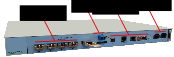
\includegraphics[scale=0.9]{Figures/mux40.pdf}
		\caption{Vista del panel frontal del \textit{muxponder} de 40Gb utilizado.}
		\label{fig:consumoagentes}
	  \end{figure}
	\end{itemize}


	\subsubsection{Justificación de elección del agente}

	Presentado el análisis y las diferencias entre ambos proyectos, en esta sección se justificará la elección de Yuma123 como servidor que se instalará en el \textit{muxponder} de 40Gb.

Como se mencionó anteriormente, Sysrepo fue la primer implementación con la que se tuvo contacto y manipulación del protocolo \textit{NETCONF}. La razón por la que se optó empezar a familiarizarse con este, fue porque se encontró una gran cantidad de ejemplos y casos de uso a la hora de realizar los módulos \textit{YANG} y relacionarlos con la instrumentación y las aplicaciones Unix. Además, la instalación del proyecto en una computadora de escritorio fue sencilla (debido a la extensa documentación y las diferentes alternativas de instalación que brinda como ser \textit{dockers}, \textit{scripts} de instalación, etc).

Sin embargo, no resultó de igual forma a la hora de realizar la compilación cruzada. La razón se debe a que Sysrepo tiene gran cantidad de dependencias como ser \textit{libyang, Google Protocol Buffers, protobuf-c, libev,} entre otros []. Específicamente, se tuvo problemas para compilar la librería \textit{“protobuf-c”} para la arquitectura \textit{NIOS}, por lo que se abandonó el uso de esta herramienta. Además, como se vio anteriormente, la demanda de memoria principal y secundaria en Sysrepo excede a los recursos disponibles en el muxponder.

En el caso de Yuma123 se logró compilar e instalar de manera correcta todas las librerías requeridas. Además, se realizaron scripts que facilitan esta tarea para las siguientes arquitecturas: \textit{ARM, NIOS y $x86_64$}. Por último, se destaca la herramienta yangdump brindada por Yuma123, la cual facilita el desarrollo de las librerías \textit{SIL} en C.

De esta forma, el factor determinante a la hora de elegir entre las distintas implementaciones \textit{NETCONF}, fue tener en cuenta las limitaciones técnicas del equipo, siendo Yuma123 el agente que mejor se adaptó a las mismas. 

% % Chapter Template

\chapter{Medologías y Herramientas de Trabajo} % Main chapter title
% cSpell:words resizebox \textit{onosapi} usecase Mcast enrutamiento parencite includegraphics pcktprocactiv lstlisting iperf

\label{Chapter5} % Change X to a consecutive number; for referencing this chapter elsewhere, use 
% \ref{ChapterX} 
En la actualidad, existen diversas metodologías para el desarrollo del software separadas en dos grandes grupos: metodologías tradicionales y metodologías ágiles. 

Será importante definir y adoptar alguna de ellas con el fin de establecer convenciones para el desarrollo del proyecto integrador. Se aborda así en la primer sección de este capítulo, la metodología de trabajo utilizada en las diferentes etapas.

Luego, se definen las herramientas de trabajo empleadas durante el desarrollo del proyecto y finalmente se describe la planificación de riesgos.

%----------------------------------------------------------------------------------------
%	SECTION 1
%----------------------------------------------------------------------------------------

\section{Metodología de desarrollo de software}
Para la gestión del desarrollo del software de este proyecto, se utilizó la metodología ágil iterativa e incremental. Dicha metodología consiste en dividir el proyecto en iteraciones bien definidas. En cada una de estas iteraciones se agregan nuevas funcionalidades y también se pueden introducir mejoras sobre las iteraciones anteriores. Los factores determinantes para la decisión de esta metodología se listan a continuación:

\begin{itemize}
	\item Existe la necesidad de tener una metodología en la cual se realicen reportes al director y co-director del proyecto, quienes analizarán los avances.
	\item Al dividir el proyecto en etapas, permite centrar la atención y organización a una pequeña parte de la misma.
	\item La necesidad de tener una metodología que sea flexible ante requerimientos cambiantes.
\end{itemize}
%-----------------------------------
%	SUBSECTION 1
%-----------------------------------

\subsection{Organización de las iteraciones}
Una vez definida la metodología para la gestión del proyecto, se definieron en conjunto con el director y co-director las iteraciones que conformarán el proyecto. Las mismas se presentan a continuación.
\begin{itemize}
	\item \textbf{Iteración 1: Familiarización con el \textit{muxponder}.} El objetivo de esta iteración es entender cómo funciona el equipo, sus capacidades, aplicaciones y utilidades.
	\item \textbf{Iteración 2: Investigación del protocolo \textit{NETCONF}.} Esta iteración tiene como objetivo realizar un estudio sobre el protocolo \textit{NETCONF}, las distintas implementaciones disponibles y cómo utilizar las mismas.
	\item \textbf{Iteración 3: Adaptación del agente \textit{NETCONF} al \textit{muxponder}.} Esta etapa del proyecto consiste en adaptar algún agente al equipo, realizando pruebas sobre las funcionalidades, capacidades y limitaciones del mismo.
	\item \textbf{Iteración 4: Realización de la librería en el \textit{muxponder}.} Independientemente del agente utilizado en el equipo, se deberá realizar una aplicación que relacione el agente \textit{NETCONF} con la instrumentación del \textit{muxponder}.
	\item \textbf{Iteración 5: Desarrollo del \textit{driver} en el controlador.} El objetivo de esta iteración será la de realizar un \textit{driver} en el controlador para que el mismo pueda comunicarse con los diferentes \textit{muxponders} presentes en la topología.
	\item \textbf{Iteración 6: Realización de la aplicación API REST en el controlador.} En esta etapa, se desarrolla la aplicación \textit{REST} que expone las distintas funcionalidades implementadas en el \textit{driver} del controlador, para que aplicaciones externas puedan hacer uso del mismo.
	\item \textbf{Iteración 7: Desarrollo de la interfaz gráfica.} Finalmente en esta iteración se desarrolla la interfaz gráfica, la cual a través de la API REST desarrollada, se comunica con los diferentes equipos haciendo uso del controlador y las bondades de \textit{SDN}.
\end{itemize}

\section{Lenguajes de programación}
En el presente trabajo de fin de grado, se utilizaron diversos lenguajes de programación. Se presenta a continuación una lista de los lenguajes empleados como así también la etapa en la cual fueron aplicados. 

\begin{itemize}
	\item \textbf{C}. El agente Yuma123 y la librería en C que comunica la instrumentación del dispositivo con el agente, se encuentran desarrollados en dicho lenguaje.  
	\item \textbf{Java}. Tanto el controlador \textit{ONOS}, como el \textit{driver} y la \textit{API REST} que se desarrolló, se encuentran escritos en dicho lenguaje. 
	\item \textbf{Python}. Durante el diseño de la interfaz gráfica, se optó por \textit{Flask} como \textit{web server}, el cual consiste en un \textit{framework} minimalista escrito en \textit{Python} que permite crear aplicaciones \textit{web} de forma rápida y sencilla. 
\end{itemize}

\section{Herramientas de desarrollo}
Las herramientas que conforman el entorno de desarrollo se listan a continuación.

\begin{itemize}
	\item \textbf{IntelliJ IDEA} como entorno de desarrollo utilizado para proyectos \textit{Java} y \textit{Python}.  
	\item \textbf{Mavenen} para la gestión de proyectos \textit{Java}, empleado especificamente en la construcción del controlador \textit{ONOS}.
	\item \textbf{Visual Studio Code} como editor de código fuente, utilizado en multiples etapas del proyecto.
\end{itemize}

\section{Control de versiones}
Se optó por utilizar el sistema de control de versiones conocido como \textit{Git} \parencite{gitref} alojado en un servidor de \textit{GitHub} \parencite{githubref}. El hecho de utilizar un sistema de control de versiones supone las siguientes ventajas:

\begin{itemize}
	\item Mantiene un historial de versiones del software. De esta forma, cada cambio se encuentra versionado permitiendo que en cualquier momento se pueda regresar el código a estados anteriores o comparar los cambios entre las distintas versiones del mismo.   
	\item Acceso remoto al proyecto. Al utilizar un servidor de \textit{Git} público, el proyecto puede ser accedido de forma remota desde cualquier equipo para continuar con el desarrollo del mismo en cualquier momento.
	\item Utilización de un esquema de ramas. Permite trabajar de manera paralela sobre diferentes partes del proyecto sin interferencias, permitiendo integrar nuevas funcionalidades al software de manera segura.
\end{itemize}

\section{Planificación de riesgos}
Todo desarrollo de software implica una serie de riesgos e incertidumbres que deben ser planificadas para definir una forma estructurada de actuar ante ellas, con el fin de cumplir con los tiempos establecidos.

El objetivo es identificar y analizar los riesgos que se puedan presentar para establecer estrategias de control y resolución que permitan ejercer una correcta supervisión de los mismos.

Por lo tanto, el proceso de gestión de riesgos está compuesto por los siguientes \textit{items}:

\begin{itemize}
	\item Identificación del riesgo.
  \item Evaluación de su probabilidad de aparición.
  \item Estimación del impacto.
  \item Establecer un plan de contingencia en caso de que ocurra.
\end{itemize}

\subsection{Criterio}
A continuación se explica el criterio utilizado para el análisis de riesgos. Los riesgos deben ser clasificados según su probabilidad de ocurrencia y los efectos que produzcan en función a los retrasos en los plazos del proyecto. 

De esta forma, se tiene la figura \ref{fig:probabilidad_riesgo} la cual describe el criterio utilizado para la probabilidad de ocurrencia de los riesgos.

\begin{figure}[H]
  \centering
  \includegraphics[scale=0.53]{Figures/caso_uso_admin.pdf}
  \caption{Probabilidad de ocurrencia del riesgo.}
  \label{fig:probabilidad_riesgo}
\end{figure}

Mientras que la figura \ref{fig:efectos_riesgo} describe el criterio que se utilizó para definir el impacto de los efectos del riesgo. 

\begin{figure}[H]
  \centering
  \includegraphics[scale=0.53]{Figures/caso_uso_admin.pdf}
  \caption{Impacto de los efectos del riesgo.}
  \label{fig:efectos_riesgo}
\end{figure}

Al combinar la probabilidad de aparición y los efectos del riesgo, se obtiene un nivel de exposición del riesgo. Esta última se puede ver de forma gráfica en la figura \ref{fig:niveles_riesgo}. 

\begin{figure}[H]
  \centering
  \includegraphics[scale=0.53]{Figures/caso_uso_admin.pdf}
  \caption{Impacto de los efectos del riesgo.}
  \label{fig:niveles_riesgo}
\end{figure}

Por otra parte, la figura \ref{fig:expo_riesgo} es utilizada como referencia para interpretar la exposición del riesgo.

\begin{figure}[H]
  \centering
  \includegraphics[scale=0.53]{Figures/caso_uso_admin.pdf}
  \caption{Referencia exposición del riesgo.}
  \label{fig:expo_riesgo}
\end{figure}
% % Chapter Template

\chapter{Validación y Verificación} % Main chapter title
% cSpell:disable
\label{Chapter5} % Change X to a consecutive number; for referencing this chapter elsewhere, use \ref{ChapterX}

% cSpell:enable
% cSpell:words resizebox \textit{onosapi} usecase Mcast enrutamiento parencite includegraphics pcktprocactiv lstlisting createmcast ssmprotocol

En el capítulo anterior se explica y caracteriza el diseño de las diferentes aplicaciones que conforman el sistema. A fines de validar su funcionamiento, será necesario poner a prueba los requerimientos de cada una de las aplicaciones desarrolladas. 

De esta forma, este capítulo propone una serie de casos de prueba determinantes para verificar el funcionamiento del proyecto. 

En primer lugar, se pondrá a prueba el agente Yuma123 instalado en el dispositivo. Luego, se verifica el funcionamiento del \textit{driver} desarrollado en el controlador \textit{ONOS}. Por último, se pone a prueba tanto la interfaz \textit{REST} como la interfaz gráfica desarrollada.

%----------------------------------------------------------------------------------------
%	SECTION 1
%----------------------------------------------------------------------------------------

\section{Verificación del agente \textit{NETCONF}}

En esta sección se pondrá a prueba el agente que se instaló en el dispositivo. Para ello, las evaluaciones realizadas tendrán como objetivo asegurar el cumplimiento de los requerimientos vistos en la figura \ref{fig:req_netconf}.

\subsection{Escenario}

La figura \ref{fig:test_topo_netconf} muestra la topología utilizada para las pruebas. Se tendrá una computadora de propósito general conectada a la interfaz de control del \textit{muxponder}. Por otra parte, el \textit{muxponder} ejecutará el agente 'netconfd' de Yuma123 mientras que el \textit{host} ejecutará el cliente 'yangcli', también de Yuma123.

\begin{figure}[!h]
	\centering
	\includegraphics[scale=0.8]{Figures/topologiatestnetconf.pdf}
	\caption{Topología utilizada para las pruebas relativas a la integración del protocolo \textit{NETCONF}.}
	\label{fig:test_topo_netconf}
  \end{figure}

  \newpage

Además, para poder poner a prueba la integración del protocolo con el dispositivo se realizan las siguientes suposiciones y condiciones previas:

\begin{itemize}
	\item El \textit{host} y el \textit{muxponder} deben tener conectividad entre sí.
    \item Se debe tener instalado en el \textit{host}, el cliente 'yangcli'.
    \item Tener instalado en el \textit{muxponder}, el agente 'netconfd'.
    \item Tanto el módulo \textit{YANG} como la librería desarrollada para el \textit{muxponder}, deben estar instalados en el mismo.
    \item La aplicación 'monitor' debe estar iniciada en el \textit{muxponder}.
    \item El equipo no debe tener ninguna configuración previa aplicada.
\end{itemize}

\subsection{Matriz de trazabilidad}

Se conformarán tres casos de pruebas. El primero tiene como objetivo verificar el inicio de sesión entre el cliente y el servidor \textit{NETCONF}. Por otra parte, la segunda prueba consiste en obtener el valor de cualquier variable visible en 'monitor'. Por último, se pone a prueba realizar un cambio en la configuración del equipo.

De esta forma, la matriz de trazabilidad resultante es la que se observa en el cuadro \ref{tab:matriz_netconf}.

\begin{table}[!h]
    \centering
    \begin{tabular}{|c|c|c|c|}
    \hline
                  & \textbf{T-R-01} & \textbf{T-R-02} & \textbf{T-R-03} \\ \hline
    \textbf{R-07} & \textit{X}      & \textit{X}      & \textit{X}      \\ \hline
    \textbf{R-08} & \textit{}       & \textit{X}      & \textit{}       \\ \hline
    \textbf{R-09} & \textit{}       & \textit{}       & \textit{X}      \\ \hline
    \textbf{R-10} & \textit{}       & \textit{}       & \textit{X}      \\ \hline
    \end{tabular}
    \caption{Matriz de trazabilidad - Verificación del protocolo \textit{NETCONF}}
    \label{tab:matriz_netconf}
\end{table}


\subsection{Casos de prueba y resultados}

A continuación, se describirán los procedimientos llevados a cabo para probar esta pieza de software. Algunos de los casos de pruebas pueden estar acompañados por imágenes para esclarecer su funcionamiento.

%----------------------------------------------------------------------------------------
\subsubsection{Caso de Prueba T-R-01}
Se pondrá a prueba el inicio de la sesión \textit{NETCONF} entre el cliente y el servidor. El cuadro \ref{tab:TR01} presenta la descripción, los procedimientos y los resultados del mismo. 

\begin{table}[H]
\rowcolors{2}{white!10!gray!80}{white!80!gray!40}
\centering
\begin{tabular}{ |m{2.5cm}|m{11cm}|  }
\hline
\multicolumn{2}{|c|}{ \textbf{ID T-R-01} } \\
\hline
\centering
\textbf{Título} & Inicio de sesión en \textit{NETCONF}. \\
\hline
\centering
\textbf{Objetivo} & Poder conectarse desde el cliente \textit{NETCONF} al servidor instalado en el \textit{muxponder}.  \\
\hline
\centering
\textbf{Procedimiento} & \begin{itemize}
  \item En el muxponder, iniciar el agente \textit{NETCONF}.   
  \item En el host, haciendo uso de la \textit{CLI} del cliente 'yangcli', indicar usuario \textit{SSH}, \textit{password}, dirección IP y puerto para iniciar sesión en el servidor \textit{NETCONF} del dispositivo.
\end{itemize}     \\
\hline
\centering
\textbf{Resultados esperados} & 
Se debe observar el proceso de intercambio de capacidades entre el cliente y el servidor. 
Una vez finalizado dicho intercambio, deben quedar habilitadas las operaciones \textit{RPC} que describe tanto el protocolo como el módulo \textit{YANG} instalado en el dispositivo.
  \\

  \hline
\centering
  \textbf{Estado}    & APROBADO  \\
\hline
\end{tabular}

\caption{Caso de Prueba T-R-01}
\label{tab:TR01}
\end{table}



%----------------------------------------------------------------------------------------
  \subsubsection{Caso de Prueba T-R-02}
  En este caso, se pone a prueba las consultas por los datos de estado y de configuración del módulo \textit{YANG}. Los procedimientos para esta prueba y sus resultados se presentan en el cuadro \ref{tab:TR02}. 

  \begin{table}[H]
    \rowcolors{2}{white!10!gray!80}{white!80!gray!40}
    \centering
    \begin{tabular}{ |m{2.5cm}|m{11cm}|  }
    \hline
    \multicolumn{2}{|c|}{ \textbf{ID T-R-02} } \\
    \hline
    \centering
    \textbf{Título} & Monitoreo de datos en \textit{NETCONF}. \\
    \hline
    \centering
    \textbf{Objetivo} & Obtener información sobre las variables de estado y de configuración del dispositivo.  \\
    \hline
    \centering
    \textbf{Procedimiento} & \begin{itemize}
      \item Iniciar sesión entre un cliente y servidor \textit{NETCONF}, tal como se describió en T-R-01.   
      \item Desde el cliente, realizar consultas con las \textit{RPC get} y \textit{get-config} al contenedor \textit{mux-state-XFP1} y \textit{mux-config} respectivamente.
    \end{itemize}     \\

    \hline
    \centering
    \textbf{Resultados esperados} & 
    El servidor deberá responder, para el primer caso, valores idénticos a los que presente el binario 'monitor' respecto al módulo XFP1. 
Para el segundo caso, el servidor deberá retornar los valores de los datos de configuración que tenga el \textit{datastore running}.
\\
    
      \hline
    \centering
      \textbf{Estado}    & APROBADO  \\
    \hline
    \end{tabular}
    
    \caption{Caso de Prueba T-R-02}
    \label{tab:TR02}
    \end{table}

  Por otra parte, la figura \ref{fig:test2_consulta} ejemplifica el resultado de una operación de consulta al \textit{container} \textit{mux-state-XFP1}, el cual contiene información de estado de dicho módulo XFP.

  \begin{figure}[H]
	\centering
	\includegraphics[scale=0.6]{Figures/test2_consulta.png}
	\caption{Consulta al \textit{container} \textit{mux-state-XFP1}.}
	\label{fig:test2_consulta}
  \end{figure}


  %----------------------------------------------------------------------------------------
  \subsubsection{Caso de Prueba T-R-03}
  Del mismo modo, el cuadro \ref{tab:TR03} detalla los procedimientos que se siguieron para verificar el funcionamiento de la  \textit{RPC} 'mux-apply-config' y las notificaciones. Cabe destacar que como se aclaró en las suposiciones para las pruebas, el equipo no se encuentra configurado. Por lo tanto se tendrán alarmas referidas a la transmisión y la recepción, entre otras. 


  \begin{table}[H]
    \rowcolors{2}{white!10!gray!80}{white!80!gray!40}
    \centering
    \begin{tabular}{ |m{2.5cm}|m{11cm}|  }
    \hline
    \multicolumn{2}{|c|}{ \textbf{ID T-R-03} } \\
    \hline
    \centering
    \textbf{Título} & Prueba de cambio de configuración y notificaciones en \textit{NETCONF}. \\
    \hline
    \centering
    \textbf{Objetivo} & Poder realizar un cambio en la configuración del dispositivo a través de la \textit{RPC} 'mux-apply-config' y verificar el funcionamiento de las notificaciones implementadas en el módulo \textit{YANG}.  \\
    \hline
    \centering
    \textbf{Procedimiento} & \begin{itemize}
      \item Iniciar sesión entre un cliente y servidor \textit{NETCONF}, tal como se describió en T-R-01.
      \item Desde el cliente \textit{NETCONF}, enviar un mensaje al servidor con la \textit{RPC} 'create-subscription'.
      \item Desde el cliente \textit{NETCONF}, enviar un mensaje al servidor con la \textit{RPC} 'mux-apply-config', para que el mismo aplique la configuración que se encuentra en el \textit{datastore running}.
    \end{itemize}     \\
    \hline
    \centering
    \textbf{Resultados esperados} & 
    En primer lugar, se espera que el cliente se suscriba correctamente a las notificaciones, recibiendo un mensaje \textit{OK} de parte del servidor. 
Además, luego de que se envíe la \textit{RPC} 'mux-apply-config' y se termine de aplicar la configuración en el equipo, en el cliente 'yangcli' se debe observar el ingreso de las notificaciones debido a que las alarmas del equipo cambiaron de estado, producto de la configuración aplicada. 
      \\
    
      \hline
    \centering
      \textbf{Estado}    & APROBADO  \\
    \hline
    \end{tabular}
    
    \caption{Caso de Prueba T-R-03}
    \label{tab:TR03}
    \end{table}


  La figura \ref{fig:test3_consulta} muestra en primer lugar cómo el cliente se suscribe a las notificaciones mediante la  \textit{RPC} 'create-suscription'. Luego, se puede observar el envío de la  \textit{RPC} 'mux-apply-config'. Seguidamente se muestran las notificaciones entrantes, producto del cambio de estado de las alarmas presentes en el equipo.
  
  \begin{figure}[H]
	\centering
	\includegraphics[scale=0.6]{Figures/test3_consulta.png}
	\caption{Suscripción y  \textit{RPC} 'mux-apply-config'.}
	\label{fig:test3_consulta}
  \end{figure}



  %----------------------------------------------------------------------------------------
%	SECTION 2
%----------------------------------------------------------------------------------------

\section{Verificación del \textit{driver}}

A continuación, en este ensayo se comprueba el funcionamiento del \textit{driver} desarrollado para el controlador \textit{ONOS}. Los requerimientos que se deben asegurar su cumplimiento son los que se observan en la figura \ref{fig:req_driver}. 

\subsection{Escenario}

En este caso, la topología utilizada para las pruebas es la que se muestra en la figura \ref{fig:test_topo_driver}. Se tendrán dos \textit{muxponders} conectados entre sí a través de las interfaces de línea de los mismos. Por otra parte, el controlador \textit{ONOS} estará conectado a la interfaz de control de ambos dispositivos. 


\begin{figure}[!h]
	\centering
	\includegraphics[scale=0.8]{Figures/topologiatestdriver.pdf}
	\caption{Topología utilizada para las pruebas relativas al \textit{driver}.}
	\label{fig:test_topo_driver}
  \end{figure}


  Además, se realizan las siguientes suposiciones:

\begin{itemize}
	\item Los agentes 'netconfd' se encuentran iniciados en ambos dispositivos.
    \item Tanto el módulo \textit{YANG} como la librería en \textit{C} desarrollada para los \textit{muxponders}, están instaladas en los mismos.
    \item La aplicación 'monitor' está iniciada en ambos \textit{muxponders}.
    \item Los dispositivos no tienen una configuración previa instalada. 
    \item Los equipos no tienen información relacionada a la presencia de vecinos.
\end{itemize}

\subsection{Matriz de trazabilidad}

A fines de poner a prueba el cumplimiento de los requerimientos para esta pieza de software, se desarrollan dos casos de prueba. 

En el primero, se verifica que el controlador sea capaz de descubrir correctamente la información de los dispositivos agregados a la topología, a través de la función \textit{DeviceDescriptionDiscovery}. La segunda prueba abarca la verificación tanto de la función \textit{LinkDiscovery} como la  \textit{RPC} 'mux-apply-config'. Además, para ambas pruebas se utilizan los comandos \textit{CLI} implementados en el \textit{driver}.

De esta forma resulta la matriz de trazabilidad que se observa en el cuadro \ref{tab:matriz_driver}.


\begin{table}[!h]
    \centering
    \begin{tabular}{|c|c|c|}
        \hline
        \textbf{}     & \textbf{T-R-04} & \textbf{T-R-05} \\ \hline
        \textbf{R-11} & \textit{X}      & \textit{}       \\ \hline
        \textbf{R-12} & \textit{}       & \textit{X}      \\ \hline
        \textbf{R-13} & \textit{}       & \textit{X}      \\ \hline
        \textbf{R-14} & \textit{X}      & \textit{X}      \\ \hline
        \end{tabular}
    \caption{Matriz de trazabilidad - Verificación del \textit{driver}}
    \label{tab:matriz_driver}
\end{table}

\subsection{Casos de prueba y resultados}

  %----------------------------------------------------------------------------------------
\subsubsection{Caso de Prueba T-R-04}

Se pondrá a prueba la función llamada \textit{DeviceDescriptionDiscovery}, la cual como se explicó en el capítulo anterior \ref{driverr}, es la encargada de registrar en el controlador información adicional de los equipos. Tanto la descripción como los procedimientos llevados a cabo y los resultados de los mismos se presentan en el cuadro \ref{tab:TR04}. 

\begin{table}[H]
  \rowcolors{2}{white!10!gray!80}{white!80!gray!40}
  \centering
  \begin{tabular}{ |m{2.5cm}|m{11cm}|  }
  \hline
  \multicolumn{2}{|c|}{ \textbf{ID T-R-04} } \\
  \hline
  \centering
  \textbf{Título} & Prueba de añadir \textit{muxponders} a la topología de ONOS.  \\
  \hline
  \centering
  \textbf{Objetivo} & Comprobar que los dispositivos se agregan correctamente al controlador, mostrando información sobre fabricante, versión del hardware y del software, identificador único, etc.  \\
  \hline
  \centering
  \textbf{Procedimiento} & \begin{itemize}
    \item Haciendo uso del comando 'onos-netcfg', enviar al controlador un mensaje \textit{JSON} con información de los dispositivos a añadir a la topología de \textit{ONOS}.
    \item Ejecutar el comando 'devices' en la \textit{CLI} del controlador. El mismo devuelve una lista con información de todos los dispositivos agregados.
  \end{itemize}     \\
  \hline
  \centering
  \textbf{Resultados esperados} & 
  Una vez que el proceso de descubrimiento de los dispositivos haya finalizado, el comando 'devices' deberá arrojar información sobre los equipos, mostrando correctamente los datos nombrados anteriormente (información del fabricante, versión de hardware y de software e identificador único).
    \\
  
    \hline
  \centering
    \textbf{Estado}    & APROBADO  \\
  \hline
  \end{tabular}
  
  \caption{Caso de Prueba T-R-04}
  \label{tab:TR04}
  \end{table}

  Por otra parte, la figura \ref{fig:test4_consulta} muestra los dispositivos agregados a la topología de \textit{ONOS}. Al hacer click sobre cualquiera de ellos, el controlador despliega un cuadro del dispositivo seleccionado mostrando la información mencionada anteriormente.

  \begin{figure}[H]
	\centering
	\includegraphics[scale=0.5]{Figures/test4_consulta.png}
	\caption{Información de dispositivos presentes en la topología de \textit{ONOS}.}
	\label{fig:test4_consulta}
  \end{figure}

  %----------------------------------------------------------------------------------------
  \subsubsection{Caso de Prueba T-R-05}

  Este caso pone a verifica tanto la función \textit{LinkDiscovery}, la cual es la encargada de formar los enlaces entre los distintos dispositivos \ref{driverlink}, como la  \textit{RPC} 'mux-apply-config', encargada de aplicar los cambios en el dispositivo \ref{drivermux}. 
  En el cuadro \ref{tab:TR05} se detalla la descripción del caso de prueba mencionado. Se asumirá que los dispositivos ya se encuentran añadidos al controlador.
  

  \begin{table}[H]
    \rowcolors{2}{white!10!gray!80}{white!80!gray!40}
    \centering
    \begin{tabular}{ |m{2.5cm}|m{11cm}|  }
    \hline
    \multicolumn{2}{|c|}{ \textbf{ID T-R-05} } \\
    \hline
    \centering
    \textbf{Título} & Prueba de formar enlaces entre \textit{muxponders} vecinos.  \\
    \hline
    \centering
    \textbf{Objetivo} & Comprobar que el controlador muestra correctamente la información referida a los enlaces entre los dispositivos.   \\
    \hline
    \centering
    \textbf{Procedimiento} & \begin{itemize}
      \item Desde el controlador, agregar información del vecino a cada uno de los dispositivos presentes en la topología.
      \item Haciendo uso de la \textit{RPC} 'mux-apply-config', aplicar una misma configuración a todos los equipos. 
      \item Desconectar el transmisor de alguno de los \textit{muxponders}.
    \end{itemize}     \\
    \hline
    \centering
    \textbf{Resultados esperados} & 
    Al agregar a cada dispositivo la información referente a su vecino, se deberá observar en la interfaz gráfica de \textit{ONOS} que los enlaces no se forman. Esto es así ya que como los dispositivos no están configurados, existirán alarmas referidas a la transmisión y recepción, y como se explicó en el capítulo anterior el \textit{driver} no formará los enlaces si dichas alarmas están presentes. 

Luego, al enviar la \textit{RPC} 'mux-apply-config' a ambos dispositivos y una vez que se termine de aplicar la configuración, las alarmas mencionadas anteriormente deberían desaparecer. Por lo tanto, en la interfaz gráfica del controlador se debe observar los enlaces formados entre los equipos, ya que no existen alarmas relacionadas a la transmisión y recepción.
Por último, el hecho de desconectar la línea del transmisor en alguno de los dos \textit{muxponders} genera alarmas en los dispositivos, por lo que la interfaz gráfica debe mostrar un cambio en la topología debido a que el enlace no se encuentra presente.  
      \\
    
      \hline
    \centering
      \textbf{Estado}    & APROBADO  \\
    \hline
    \end{tabular}
    
    \caption{Caso de Prueba T-R-05}
    \label{tab:TR05}
    \end{table}

  La figura \ref{fig:test5_1} muestra la topología presente en el controlador una vez se le indicó a cada dispositivo la presencia de un vecino. Como se puede notar, el controlador no forma los enlaces entre los mismos ya que los dispositivos contienen alarmas debido a que no están configurados. 

  \begin{figure}[H]
	\centering
	\includegraphics[scale=0.5]{Figures/test5_1.png}
	\caption{Vista de la topología de \textit{ONOS} - Dispositivos sin configurar.}
	\label{fig:test5_1}
  \end{figure}

  A su vez, en la figura \ref{fig:test5_2} se observa que una vez aplicada la configuración en ambos dispositivos, la cantidad de alarmas presentes se reducen. Luego, al no existir alarmas referidas a la transmisión y recepción de los equipos, el controlador puede formar correctamente el enlace entre los mismos. 

  \begin{figure}[H]
	\centering
	\includegraphics[scale=0.5]{Figures/test5_2.png}
	\caption{Vista de la topología de \textit{ONOS} - Dispositivos configurados.}
	\label{fig:test5_2}
  \end{figure}

  Por último, la figura \ref{fig:test5_3} ejemplifica lo que sucede cuando se desconecta el transmisor en alguno de los dispositivos, provocando así la caída de un enlace en la topología de \textit{ONOS}.

  \begin{figure}[H]
	\centering
	\includegraphics[scale=0.5]{Figures/test5_3.png}
	\caption{Vista de la topología de \textit{ONOS} - Dispositivos configurados, con un enlace desconectado.}
	\label{fig:test5_3}
  \end{figure}



%----------------------------------------------------------------------------------------
%	SECTION 3
%----------------------------------------------------------------------------------------

\section{Verificación de la interfaz gráfica y la interfaz \textit{REST}}

Finalmente, en esta sección se pondrán a prueba ambas interfaces desarrolladas. Para ello, las pruebas realizadas tendrán como objetivo validar el cumplimiento de los requerimientos vistos en la figura \ref{fig:req_app}. 

Además, los casos de prueba presentados a continuación harán uso tanto del \textit{driver} como de la aplicación \textit{C} desarrollada para el agente \textit{NETCONF}.


\subsection{Escenario}

La topología utilizada para las pruebas mencionadas anteriormente se muestra en la figura \ref{fig:test_topo_rest}. 
Se tendrán dos \textit{muxponders} conectados entre sí a través de las interfaces de línea de los mismos. Además, el controlador \textit{ONOS} estará conectado a la interfaz de control de ambos dispositivos. Por último, se tienen dos computadoras de propósito general conectadas a los módulos XFP1 de los \textit{muxponders}.



\begin{figure}[H]
	\centering
	\includegraphics[scale=0.8]{Figures/topologiatest.pdf}
	\caption{Topología utilizada para las pruebas relativas a la interfaz gráfica e interfaz \textit{REST}.}
	\label{fig:test_topo_rest}
  \end{figure}


  Además, se realizan las siguientes suposiciones:

\begin{itemize}
	\item Los agentes 'netconfd' se encuentran iniciados en ambos dispositivos.
    \item Tanto el módulo \textit{YANG} como la librería en \textit{C} desarrollada para los \textit{muxponders}, están instaladas en los mismos.
    \item La aplicación 'monitor' está iniciada en ambos \textit{muxponders}.
    \item Los dispositivos no tienen una configuración previa instalada. 
    \item Los equipos no tienen información relacionada a la presencia de vecinos.
\end{itemize}


\subsection{Matriz de trazabilidad}

Se presenta a continuación en el cuadro \ref{tab:matriz_rest} la matriz de trazabilidad para las pruebas realizadas. 

En la primera prueba, se verifica poder agregar dispositivos a través de la interfaz gráfica y configurar a ambos como vecinos. 
Luego, se verifica en la prueba T-R-07 que puedan visualizarse las alarmas en la aplicación \textit{WEB}.
Por otra parte, en la prueba T-R-08 se comprueba que sea posible visualizar, a través de la interfaz gráfica, cualquier dato de estado de los dispositivos.
Por último, se ensaya realizar un cambio en la configuración en los dispositivos de tal forma que se permita la conectividad entre los \textit{host} A y B.
\\


\begin{table}[!h]
    \centering
    \begin{tabular}{|c|c|c|c|c|}
      \hline
      \textbf{}     & \textbf{T-R-06} & \textbf{T-R-07}    & \textbf{T-R-08} & \textbf{T-R-09} \\ \hline
      \textbf{R-15} & \textit{}       & \textit{X}         & \textit{X}      & \textit{X}      \\ \hline
      \textbf{R-16} & \textit{X}      & \textit{}          & \textit{}       & \textit{X}      \\ \hline
      \textbf{R-17} & \textit{}       & \textit{\textbf{}} & \textit{}       & \textit{X}      \\ \hline
      \textbf{R-18} & \textit{}       & \textit{X}         & \textit{}       & \textit{}       \\ \hline
      \textbf{R-19} & \textit{X}      & \textit{}          & \textit{}       & \textit{X}      \\ \hline
      \textbf{R-20} & \textit{}       & \textit{}          & \textit{}       & \textit{X}      \\ \hline
      \textbf{R-21} & \textit{}       & \textit{}          & \textit{X}      & \textit{}       \\ \hline
      \end{tabular}
    \caption{Matriz de trazabilidad - Verificación de la interfaz \textit{REST} e interfaz gráfica}
    \label{tab:matriz_rest}
\end{table}


\subsection{Casos de prueba y resultados}

\subsubsection{Caso de Prueba T-R-06}

A continuación, se asegura agregar nuevos dispositivos a la topología del controlador desde la interfaz gráfica y configurarlos como vecinos. Los procedimientos llevados a cabo para dicha prueba se observan en el cuadro \ref{tab:TR06}.


\begin{table}[H]
  \rowcolors{2}{white!10!gray!80}{white!80!gray!40}
  \centering
  \begin{tabular}{ |m{2.5cm}|m{11.5cm}|  }
  \hline
  \multicolumn{2}{|c|}{ \textbf{ID T-R-06} } \\
  \hline
  \centering
  \textbf{Título} & Añadir \textit{muxponders} a la topología de \textit{ONOS} desde la interfaz gráfica y configurarlos como vecinos.  \\
  \hline
  \centering
  \textbf{Objetivo} & Comprobar que los dispositivos se agregan correctamente al controlador haciendo uso de la interfaz gráfica y que es posible agregar información de vecinos a cada uno de ellos desde la misma.   \\
  \hline
  \centering
  \textbf{Procedimiento} & \begin{itemize}
    \item Desde la aplicación \textit{WEB}, agregar un nuevo dispositivo indicando dirección IP y puerto.
    \item Desde la aplicación \textit{WEB}, hacer click en 'TOPOLOGIA' y configurar ambos equipos como vecinos.
    \item En el controlador, ejecutar el comando 'devices'.
    \item Desde la aplicación \textit{WEB}, hacer click en 'CONFIGURACION'.
  \end{itemize}     \\
  \hline
  \centering
  \textbf{Resultados esperados} & 
  Luego de ejecutar el comando 'devices' en la \textit{CLI} del controlador, se debe mostrar la información de fabricante, versión del hardware y software e identificador único de ambos dispositivos agregados. 
Por otra parte, la sección 'CONFIGURACION' debe mostrar la información mencionada anteriormente junto con el identificador único del vecino agregado. 
  
    \\
  
    \hline
  \centering
    \textbf{Estado}    & APROBADO  \\
  \hline
  \end{tabular}
  
  \caption{Caso de Prueba T-R-06}
  \label{tab:TR06}
  \end{table}



  \subsubsection{Caso de Prueba T-R-07}

El objetivo del caso de prueba presentado en el cuadro \ref{tab:TR07}, es el de verificar que la interfaz gráfica presente de forma correcta la información relacionada a las alarmas en los dispositivos. 
Se hará uso tanto de la aplicación 'monitor' como de los comandos '\textit{alarms}' y '\textit{alarms-count}' de \textit{ONOS} para validar las alarmas presentes.


\begin{table}[H]
  \rowcolors{2}{white!10!gray!80}{white!80!gray!40}
  \centering
  \begin{tabular}{ |m{2.5cm}|m{11cm}|  }
  \hline
  \multicolumn{2}{|c|}{ \textbf{ID T-R-07} } \\
  \hline
  \centering
  \textbf{Título} & Prueba de visualización de alarmas desde la interfaz gráfica.  \\
  \hline
  \centering
  \textbf{Objetivo} & Comprobar que la aplicación \textit{WEB} muestra correctamente las alarmas de todos los \textit{muxponders} presentes en la topología.   \\
  \hline
  \centering
  \textbf{Procedimiento} & \begin{itemize}
    \item En la aplicación \textit{WEB}, hacer click sobre 'ALARMAS'.
    \item En el controlador, ejecutar los comandos 'alarms' y 'alarms-counts'. 
    \item En la \textit{CLI} de cada uno de los \textit{muxponders}, verificar con la aplicación 'monitor' la presencia de alarmas.
  \end{itemize}     \\
  \hline
  \centering
  \textbf{Resultados esperados} & 
  La cantidad de alarmas presentes anunciadas en la interfaz gráfica debe ser la misma que las anunciadas por el controlador al ejecutar el comando 'alarms-counts'.
Además, la información referida a cada alarma, como por ejemplo el dispositivo de origen y el nombre de la misma, debe ser igual a las que muestre el comando 'alarms' en el controlador \textit{ONOS}.
Finalmente, las alarmas presentes en cada dispositivo deben poder visualizarse en la aplicación 'monitor' de los \textit{muxponders} relacionados. 
    \\
  
    \hline
  \centering
    \textbf{Estado}    & APROBADO  \\
  \hline
  \end{tabular}
  
  \caption{Caso de Prueba T-R-07}
  \label{tab:TR07}
  \end{table}

  Tal como se puede ver en la figura \ref{fig:test7_1}, se tienen 12 alarmas presentes referidas a los módulos XFP2, XFP3 y XFP4 de ambos dispositivos.

  \begin{figure}[H]
	\centering
	\resizebox{\textwidth}{!}{\includegraphics{Figures/test7_1.pdf}}
	\caption{Alarmas visualizadas en la interfaz gráfica.}
	\label{fig:test7_1}
  \end{figure}

  Se puede observar lo mismo al ejecutar los comandos '\textit{alarms}' y '\textit{alarms-counts}', los cuales listan las alarmas presentes en el controlador. De esta forma, se puede ver en la figura \ref{fig:test7_2} la salida del comando '\textit{alarms-counts}', la cual anuncia la misma cantidad de alarmas presentes en el controlador.

  \begin{figure}[H]
	\centering
	\includegraphics[scale=0.5]{Figures/test7_2.png}
	\caption{Alarmas visualizadas en la \textit{CLI} del controlador.}
	\label{fig:test7_2}
  \end{figure}

  Por último, se muestra en la figura \ref{fig:test7_3} la salida del binario 'monitor' de uno de los \textit{muxponder}. En ella, es posible observar 6 etiquetas '\textit{Alarm}' en la sección de modulos XFP. Teniendo en cuenta que se tiene el mismo resultado en el otro dispositivo, se tienen las 12 alarmas en total.

  \begin{figure}[H]
	\centering
	\includegraphics[scale=0.5]{Figures/test7_3.png}
	\caption{Alarmas visualizadas en 'monitor' en uno de los \textit{muxponders}.}
	\label{fig:test7_3}
  \end{figure}

  \subsubsection{Caso de Prueba T-R-08}

  Se presenta la verificación que se observa en el cuadro \ref{tab:TR08}, la cual tiene como objetivo examinar que sea posible observar cualquier dato de estado del dispositivo a través de la interfaz gráfica. 
  
  Al igual que en la prueba anterior, se hará uso del binario 'monitor' para comprobar su funcionamiento.
  
  
  \begin{table}[H]
    \rowcolors{2}{white!10!gray!80}{white!80!gray!40}
    \centering
    \begin{tabular}{ |m{2.5cm}|m{11cm}|  }
    \hline
    \multicolumn{2}{|c|}{ \textbf{ID T-R-08} } \\
    \hline
    \centering
    \textbf{Título} & Prueba de visualización de los datos de estado desde la interfaz gráfica.  \\
    \hline
    \centering
    \textbf{Objetivo} & Verificar que desde la aplicación \textit{WEB} se pueda obtener información de los datos de estado de cada \textit{muxponder} presente en la topología.   \\
    \hline
    \centering
    \textbf{Procedimiento} & \begin{itemize}
      \item En la aplicación \textit{WEB}, hacer click sobre 'ESTADO'.
      \item En el controlador, consultar por los datos de estado de cada dispositivo presente haciendo uso del comando 'get'. 
      \item Verificar con 'monitor' los valores para los datos de estado.
    \end{itemize}     \\
    \hline
    \centering
    \textbf{Resultados esperados} & 
    La información que presenta la sección 'ESTADO' de la interfaz gráfica debe tener valores idénticos a los obtenidos por el controlador luego de ejecutar el comando 'get'.

Además, la información que muestra 'monitor' debe coincidir con la que se observa en la sección de 'ESTADO' en la aplicación \textit{WEB}.
      \\
    
      \hline
    \centering
      \textbf{Estado}    & APROBADO  \\
    \hline
    \end{tabular}
    
    \caption{Caso de Prueba T-R-08}
    \label{tab:TR08}
    \end{table}

    A continuación, en la figura \ref{fig:test8_1} se muestran los valores obtenidos por la interfaz gráfica referidos al \textit{container} '\textit{misc}' de ambos dispositivos. 

    \begin{figure}[H]
        \centering
        \resizebox{\textwidth}{!}{\includegraphics{Figures/test8_1.png}}
        \caption{Datos de estado, observados desde la interfaz gráfica.}
        \label{fig:test8_1}
      \end{figure}

      Por otra parte, se observa en la figura \ref{fig:test8_2} la sección referida a '\textit{misc}' en 'monitor', los cuales tienen los mismos valores que los obtenidos por la interfaz gráfica. Es importante aclarar que debido a la cantidad de los datos presentes en este \textit{container}, las figuras nombradas anteriormente solo muestran una porción de los datos.
      
      Por lo tanto, se observan únicamente los primeros cinco valores.

      \begin{figure}[H]
        \centering
        \begin{subfigure}[b]{0.45\textwidth}
            \centering
            \includegraphics[width=\textwidth]{Figures/test8_2_mux1.png}
            \caption{'monitor' del \textit{muxponder} '141'.}
        \end{subfigure}
        \quad
        \begin{subfigure}[b]{0.45\textwidth}  
            \centering 
            \includegraphics[width=\textwidth]{Figures/test8_2_mux2.png}
            \caption{'monitor' del \textit{muxponder} '142'.}
        \end{subfigure}
        \caption{Datos de estado, observados desde 'monitor'.}
        \label{fig:test8_2}
    \end{figure}

      \subsubsection{Caso de Prueba T-R-09}

      Por último, el caso de prueba mostrado en el cuadro \ref{tab:TR09} tiene como objetivo verificar que es posible configurar los \textit{muxponders} de tal manera que los \textit{host} A y B tengan conectividad entre sí. 

      \begin{table}[H]
        \rowcolors{2}{white!10!gray!80}{white!80!gray!40}
        \centering
        \begin{tabular}{ |m{2.5cm}|m{11cm}|  }
        \hline
        \multicolumn{2}{|c|}{ \textbf{ID T-R-09} } \\
        \hline
        \centering
        \textbf{Título} & Prueba de conectividad entre los \textit{hosts} A y B.  \\
        \hline
        \centering
        \textbf{Objetivo} & Poder configurar a través de la interfaz gráfica ambos \textit{muxponders}, con el objetivo de que los \textit{hosts} tengan conectividad entre ellos.   \\
        \hline
        \centering
        \textbf{Procedimiento} & \begin{itemize}
          \item Desde la sección 'TOPOLOGÍA' en la aplicación \textit{WEB}, configurar ambos dispositivos como vecinos.
          \item Hacer click en la sección 'PERFILES' y añadir dos perfiles, uno con tipo de tráfico 'xge' y otro con un tipo de tráfico 'otu2'.
          \item  Hacer click en 'ALTURA-MXP'. En el cuadro de configuración, aplicar a uno de los dispositivos el perfil de configuración 'xge' mientras que al otro aplicar el perfil de configuración 'otu2'.
          \item En cada uno de los \textit{hosts}, verificar si tienen conectividad entre ellos utilizando la aplicación 'ping'.
          \item Hacer click en 'CONFIGURACION'. Verificar la configuración aplicada en los dispositivos.
          \item Hacer click en 'ALTURA-MXP'. En el cuadro de configuración, seleccionar el \textit{muxponder} configurado anteriormente con el perfil 'otu2' y aplicarle ahora la configuración 'xge'.
          \item En cada uno de los \textit{hosts}, verificar si tienen conectividad entre ellos utilizando la aplicación 'ping'.

        \end{itemize}     \\
        \hline
        \centering
        \textbf{Resultados esperados} & 
        Luego de configurar a los dispositivos como vecinos y aplicar un perfil de configuración diferente a cada uno de ellos, la interfaz deberá mostrar en la sección principal una advertencia de que existen dispositivos presentes en la topología con una configuración diferente. 

        Si los \textit{muxponders} tienen aplicada una configuración diferente entre ellos, no existirá conectividad entre los host, por lo que los dispositivos no podrán realizar un 'ping' entre ellos.
 
        Luego, al configurar ambos dispositivos con el mismo perfil de configuración, la interfaz gráfica debe mostrar en la sección principal que la alarma referida a configuración inconsistente desapareció. Además, la prueba de 'ping' debe mostrar ahora que los \textit{host} pueden alcanzarse.
          \\
        
          \hline
        \centering
          \textbf{Estado}    & APROBADO  \\
        \hline
        \end{tabular}
        
        \caption{Caso de Prueba T-R-09}
        \label{tab:TR09}
        \end{table}

      La figura \ref{fig:test9_1} muestra la sección principal de la interfaz gráfica. En ella, es posible observar un recuadro en amarillo indicando que se detectó una configuración inconsistente entre los dispositivos (o sea, que los dispositivos vecinos no tienen la misma configuración). 

      \begin{figure}[H]
        \centering
        \resizebox{\textwidth}{!}{\includegraphics{Figures/test9_1.png}}
        \caption{Detección de configuración inconsistente entre dispositivos vecinos.}
        \label{fig:test9_1}
      \end{figure}

      En este estado, si los \textit{host} A y B tratan de realizar un ping entre ellos el resultado es el que se puede ver en la figura \ref{fig:test9_2}. Como se esperaba, los \textit{hosts} no tienen conectividad entre ellos debido a la configuración inconsistente aplicada a los dispositivos.

      \begin{figure}[H]
        \centering
        \includegraphics[scale=0.7]{Figures/test9_2.png}
        \caption{Prueba fallida de conectividad entre \textit{host} A y \textit{host} B.}
        \label{fig:test9_2}
      \end{figure}

      Luego, al configurar ambos dispositivos con el perfil de configuración xge, la interfaz muestra que la alarma debido a configuración inconsistente desapareció, tal como se muestra en la figura \ref{fig:test9_3}.


      \begin{figure}[H]
        \centering
        \resizebox{\textwidth}{!}{\includegraphics{Figures/test9_3.png}}
        \caption{Detección de configuración consistente entre dispositivos vecinos.}
        \label{fig:test9_3}
      \end{figure}

      Por último, se realiza nuevamente la prueba de conectividad realizando un ping entre los \textit{hosts}. Como se puede ver en la figura \ref{fig:test9_4}, los clientes ahora tienen conectividad entre ellos debido a la configuración consistente entre los dispositivos vecinos.

      \begin{figure}[H]
        \centering
        \includegraphics[scale=0.7]{Figures/test9_4.png}
        \caption{Prueba exitosa de conectividad entre \textit{host} A y \textit{host} B.}
        \label{fig:test9_4}
      \end{figure}
 
% % Chapter Template

\chapter{Diseño de la aplicación de interfaz de usuario} % Main chapter title

\label{Chapter6} % Change X to a consecutive number; for referencing this chapter elsewhere, use \ref{ChapterX}
 En este capítulo se abordará el proceso de diseño e implementación de una interfaz gráfica de usuario, cuyo objeto principal es exponer de manera sencilla las capacidades de la aplicación desarrollada en el capítulo anterior. \


 Primero se definirán los requerimientos de la aplicación, luego en base a estos se establecerán parámetros para la implementación, tales como el lenguaje de desarrollo o interfaz comunicación con el exterior.
 Una vez finalizado el desarrollo, se definirán casos de prueba y se verificará el correcto funcionamiento de la aplicación.
%----------------------------------------------------------------------------------------
%	SECTION 1
%----------------------------------------------------------------------------------------

\section{Análisis de Requerimientos}
Los requerimientos funcionales estarán dados por:
\begin{itemize}
    \item [R-01] \textit{Brindar información sobre la situación actual de la red}: se deben incluir datos que permitan identifcar los dispositivos controlados y los \textit{hosts} conectados.
    \item [R-02] \textit{Proveer información sobre el estado de la distribución de contenido}: incluyendo datos sobre las rutas \textit{multicast} creadas, las fuentes habilitadas a transmitir y los suscriptores bloqueados.
    \item [R-03] \textit{Administrar los proveedores y suscriptores habilitados}: brindar la capacidad de modificar los parámetros de la aplicación interna al controlador para permitir o bloquear algunas conexiones.
\end{itemize}


Por otro lado, se definen los siguientes requerimientos no funcionales:
\begin{itemize}
    \item [R-04] \textit{Ofrecer una interfaz gráfica amigable al usuario}: el entorno de operación debe ser sencillo de administrar.
    \item [R-05] \textit{Tiempo de actualización de la información}: Los datos en la interfaz deben actualizarse en intervalos de tiempo cortos.
\end{itemize}

%-----------------------------------
%	SECTION 2
%-----------------------------------
\section{Implementación y comunicación con el controlador}

De acuerdo a los requerimientos definidos en la sección anterior, se puede inferir que las actividades que debe desempeñar esta aplicación residen principalmente en consultas a la REST API definida como interfaz \textit{northbound} de ONOS. Se utilizará como plataforma para la implementación un servidor web, ya que brinda mayor versatilidad y simplicidad para el desarrollo de la interfaz gráfica a través de los lenguajes de programación web. 

Como se muestra en la figura \ref{fig:gui_diagram}, para el desarrollo del \textit{"front-end"}  de la interfaz se utilizará \textit{HTML} con el agregado de librerías de \textit{Bootstrap} que simplifican el diseño. Por otro lado, las funciones \textit{"back-end"} estarán implementadas en \textit{Python} un lenguaje de programación de alto nivel con librerías que facilitan la comunicación con la REST API de ONOS y la lectura de los datos. La comunicación entre el \textit{"front-end"} y  el \textit{"back-end"} se logra a través de \textit{CGI o Common Gateway Interface}.

\begin{figure}[th]
	\centering 
	\resizebox{.3\textwidth}{!}{\includegraphics{Figures/gui_diagram.png}}%
	\caption[Esquema de la interfaz de usuario]{Esquema de la interfaz de usuario.}
	\label{fig:gui_diagram}
\end{figure}


%----------------------------------------------------------------------------------------
%	SECTION 3
%----------------------------------------------------------------------------------------

\section{Validación y Verificación}

Los casos de prueba diseñados para la interfaz de usuario estan representados por los cuadros \ref{t-Situacion-actual-de-la-red}, \ref{t-Informacion-sobre-el-estado-de-distribucion-de-contenido}, \ref{t-Administrar-proveedores-y-clientes-autorizados}, \ref{t-Brindar-una-interfaz-sencilla-para-la-administracion-del-servicio} y \ref{t-Mantener-la-informacion-actualizada}. En la figura \ref{fig:gui_captura} se presenta una captura de la interfaz de usuario desarrolada.

\begin{figure}[th]
	\centering 
	\resizebox{1\textwidth}{!}{\includegraphics{Figures/gui_captura.png}}%
	\caption[Captura de la interfaz de usuario]{Captura de la interfaz de usuario.}
	\label{fig:gui_captura}
\end{figure}


\begin{table}[th]
\centering
\caption{Situación actual de la red}
\label{t-Situacion-actual-de-la-red}
\resizebox{\textwidth}{!}{%
\begin{tabular}{|c|l|}
\hline
\rowcolor[HTML]{C0C0C0} 
\textbf{Id} & \multicolumn{1}{c|}{\cellcolor[HTML]{C0C0C0}T-R-01} \\ \hline
\textbf{Título} & \multicolumn{1}{c|}{Situación actual de la red} \\ \hline
\rowcolor[HTML]{C0C0C0} 
\textbf{Objetivo} & \begin{tabular}[c]{@{}l@{}}Incluir datos sobre dispositivos controlados y los \textit{hosts} \\ conectados que permitan identificarlos y conocer su \\ estado de conexión.\end{tabular} \\ \hline
\textbf{Procedimiento} & \begin{tabular}[c]{@{}l@{}}1. Conectar y desconectar un \textit{host}.\\ 2. Conectar y desconectar un dispositivo.\end{tabular} \\ \hline
\rowcolor[HTML]{C0C0C0} 
\textbf{Resultados Esperados} & \begin{tabular}[c]{@{}l@{}}Para el caso 1, se visualiza primero la conexión de un \\ nuevo \textit{host} y luego la desconexión de este mismo. El \\ resultado es análogo para el caso 2.\end{tabular} \\ \hline
\textbf{Estado} & \multicolumn{1}{c|}{Aprobado} \\ \hline
\end{tabular}%
}
\end{table}

% Please add the following required packages to your document preamble:
% \usepackage{graphicx}
% \usepackage[table,xcdraw]{xcolor}
% If you use beamer only pass "xcolor=table" option, i.e. \documentclass[xcolor=table]{beamer}
\begin{table}[th]
\centering
\caption{Información sobre el estado de distribución de contenido}
\label{t-Informacion-sobre-el-estado-de-distribucion-de-contenido}
\resizebox{\textwidth}{!}{%
\begin{tabular}{|c|l|}
\hline
\rowcolor[HTML]{C0C0C0} 
\textbf{Id} & \multicolumn{1}{c|}{\cellcolor[HTML]{C0C0C0}T-R-02} \\ \hline
\textbf{Título} & \multicolumn{1}{c|}{Información sobre el estado de distribución de contenido} \\ \hline
\rowcolor[HTML]{C0C0C0} 
\textbf{Objetivo} & \begin{tabular}[c]{@{}l@{}}Proveer información acerca de las rutas \textit{multicast} creadas, \\ las fuentes habilitadas a transmitir y los suscriptores bloqueados.\end{tabular} \\ \hline
\textbf{Procedimiento} & \begin{tabular}[c]{@{}l@{}}1. Establecer una sola ruta \textit{multicast} con su proveedor de \\ contenido y sus respectivos clientes.\\ 2. Establecer otra ruta \textit{multicast} con su proveedor de \\ contenido y sus respectivos clientes, pero bloqueando a \\ un \textit{host}.\\ 3. Desbloquear dicho \textit{host} para esa ruta.\end{tabular} \\ \hline
\rowcolor[HTML]{C0C0C0} 
\textbf{Resultados Esperados} & \begin{tabular}[c]{@{}l@{}}En el caso 1, la interfaz de usuario muestra solo 1 fuente \\ habilitada a transmitir al grupo \textit{multicast} correspondiente y la \\ IP de los clientes suscriptos. Para el caso 2, para esta nueva ruta \\ se visualiza un nuevo proveedor autorizado, una nueva lista de \\ clientes suscriptos y clientes bloqueados. Finalmente, este último \\ cliente desaparece de la lista de bloqueados de dicha ruta \textit{multicast}.\end{tabular} \\ \hline
\textbf{Estado} & \multicolumn{1}{c|}{Aprobado} \\ \hline
\end{tabular}%
}
\end{table}

% Please add the following required packages to your document preamble:
% \usepackage{graphicx}
% \usepackage[table,xcdraw]{xcolor}
% If you use beamer only pass "xcolor=table" option, i.e. \documentclass[xcolor=table]{beamer}
\begin{table}[th]
\centering
\caption{Administrar proveedores y clientes autorizados}
\label{t-Administrar-proveedores-y-clientes-autorizados}
\resizebox{\textwidth}{!}{%
\begin{tabular}{|c|l|}
\hline
\rowcolor[HTML]{C0C0C0} 
\textbf{Id} & \multicolumn{1}{c|}{\cellcolor[HTML]{C0C0C0}T-R-03} \\ \hline
\textbf{Título} & \multicolumn{1}{c|}{Administrar proveedores y clientes autorizados} \\ \hline
\rowcolor[HTML]{C0C0C0} 
\textbf{Objetivo} & \begin{tabular}[c]{@{}l@{}}Modificar los parámetros de la aplicación interna al controlador \\ para permitir o bloquear proveedores y clientes\end{tabular} \\ \hline
\textbf{Procedimiento} & \begin{tabular}[c]{@{}l@{}}1. Bloquear un cliente que está recibiendo tráfico de un grupo \\ \textit{multicast} determinado.\\ 2. Desbloquear el cliente.\\ 3. Bloquear una fuente que está transmitiendo y hay \textit{hosts} \\ escuchando.\\ 4. Autorizar la fuente a transmitir a un grupo determinado.\end{tabular} \\ \hline
\rowcolor[HTML]{C0C0C0} 
\textbf{Resultados Esperados} & \begin{tabular}[c]{@{}l@{}}En primer lugar, se observa como el cliente pasa de la lista de \\ autorizados a la de bloqueados de dicha ruta \textit{multicast}. Segundo, \\ se produce la acción contraria. Por otro lado, en el caso 3 la fuente \\ desaparece de la lista de proveedores autorizados y la información \\ de la ruta \textit{multicast} a la que pertenecía desaparece. Para el caso 4, \\ la fuente vuelve a la lista de autorizados y la información de la ruta \\ \textit{multicast} se restaura.\end{tabular} \\ \hline
\textbf{Estado} & \multicolumn{1}{c|}{Aprobado} \\ \hline
\end{tabular}%
}
\end{table}

% Please add the following required packages to your document preamble:
% \usepackage{graphicx}
% \usepackage[table,xcdraw]{xcolor}
% If you use beamer only pass "xcolor=table" option, i.e. \documentclass[xcolor=table]{beamer}
\begin{table}[th]
\centering
\caption{Brindar una interfaz sencilla para la administración del servicio}
\label{t-Brindar-una-interfaz-sencilla-para-la-administracion-del-servicio}
\resizebox{\textwidth}{!}{%
\begin{tabular}{|c|c|}
\hline
\rowcolor[HTML]{C0C0C0} 
\textbf{Id} & T-R-04 \\ \hline
\textbf{Título} & Brindar una interfaz sencilla para la administración del servicio \\ \hline
\rowcolor[HTML]{C0C0C0} 
\textbf{Objetivo} & \begin{tabular}[c]{@{}c@{}}El entorno para la administración de la red debe ser organizado y \\ sencillo de operar.\end{tabular} \\ \hline
\textbf{Procedimiento} & \multicolumn{1}{l|}{1. Realizar una serie de operaciones aleatorias con la interfaz.} \\ \hline
\rowcolor[HTML]{C0C0C0} 
\textbf{Resultados Esperados} & \multicolumn{1}{l|}{\cellcolor[HTML]{C0C0C0}\begin{tabular}[c]{@{}l@{}}Toda la información se presenta en una sola vista, dónde también \\ se muestran los campos para realizar los cambios de las \\ configuraciones del servicio. A su vez, con un máximo de 2 clicks \\ el usuario puede realizar cualquiera de las operaciones.\end{tabular}} \\ \hline
\textbf{Estado} & Aprobado \\ \hline
\end{tabular}%
}
\end{table}

% Please add the following required packages to your document preamble:
% \usepackage{graphicx}
% \usepackage[table,xcdraw]{xcolor}
% If you use beamer only pass "xcolor=table" option, i.e. \documentclass[xcolor=table]{beamer}
\begin{table}[th]
\centering
\caption{Mantener la información actualizada}
\label{t-Mantener-la-informacion-actualizada}
\resizebox{\textwidth}{!}{%
\begin{tabular}{|c|c|}
\hline
\rowcolor[HTML]{C0C0C0} 
\textbf{Id} & T-R-05 \\ \hline
\textbf{Título} & Mantener la información actualizada \\ \hline
\rowcolor[HTML]{C0C0C0} 
\textbf{Objetivo} & \begin{tabular}[c]{@{}c@{}}Los datos en la interfaz deben actualizarse cada un \\ tiempo acorde a los intervalos entre los distintos eventos de la red\end{tabular} \\ \hline
\textbf{Procedimiento} & \multicolumn{1}{l|}{\begin{tabular}[c]{@{}l@{}}1. Realizar una serie de cambios en las configuraciones del servicio.\\ 2. Desconectar y conectar \textit{hosts} y dispositivos de red.\end{tabular}} \\ \hline
\rowcolor[HTML]{C0C0C0} 
\textbf{Resultados Esperados} & \multicolumn{1}{l|}{\cellcolor[HTML]{C0C0C0}\begin{tabular}[c]{@{}l@{}}Los cambios en las configuraciones y en el estado de conexión de los \\ \textit{hosts} y los \textit{switches} se refrescan en intervalos de tiempo no mayor \\ a 10 segundos.\end{tabular}} \\ \hline
\textbf{Estado} & Aprobado \\ \hline
\end{tabular}%
}
\end{table} 
% % Chapter Template

\chapter{Conclusión} % Main chapter title

\label{Chapter7} % Change X to a consecutive number; for referencing this chapter elsewhere, use \ref{ChapterX}
En este proyecto, se ha realizado una vasta investigación para adquirir conocimientos relacionados particularmente con la gestión de la configuración de los equipos de red y también con el esquema denominado Redes Definidas por Software. Así, se realizó una comparación entre dos implementaciones abiertas del protocolo \textit{NETCONF} y un estudio del controlador \textit{ONOS}. Luego, se propuso utilizar ambas tecnologías con el fin de poder monitorear y configurar un dispositivo óptico, precisamente un \textit{muxponder} de 40GB. Para materializar esto, se construyó un ambiente de trabajo conformado por el controlador \textit{ONOS}, \textit{switchs} virtuales, computadoras de propósito general e integrando el agente \textit{NETCONF} \textit{Yuma123} en el \textit{muxponder} de 40GB.

A continuación, se listan las principales reflexiones finales obtenidas tras el desarrollo de este proyecto.

\begin{itemize}

    % investigación sobre SDN, creamos un documento
    \item Al finalizar este trabajo, se adquirió un conocimiento acabado del nuevo esquema de red que plantea  \textit{SDN}. Se ha generado un documento donde se recopilan todas las características, el principio de funcionamiento y beneficios de este innovador y prometedor enfoque. A su vez, este escrito contiene un análisis del controlador \textit{ONOS}, mostrando su diseño y como implementa este las diversas cualidades de un controlador  \textit{SDN}.

    % uso de netconf
    \item En el proyecto integrador se ha realizado un estudio sobre la gestión de la configuración de los equipos de red. Se logró integrar y adaptar al \textit{muxponder} una implementación de código abierto del protocolo \textit{NETCONF} llamada Yuma123. 
    
    \item Con el fin de poder administrar la configuración del equipo, se realizó un módulo \textit{YANG} que describe y modela los datos del dispositivo. También fue necesario realizar una librería en \textit{C} que relacione los comportamientos típicos y las variables del equipo con el agente Yuma123.
        
    % uso del controlador ONOS
    \item Para lograr una comunicación entre los dispositivos y el controlador, se desarrolló un \textit{driver} en la interfaz \textit{southbound} de \textit{ONOS}. Además, se realizó también una aplicación que reside en la interfaz \textit{northbound} del mismo, con el fin de exponer interfaces a las aplicaciones externas para que estas puedan comunicarse con los dispositivos. 

    % nodo físico
    \item Haciendo uso de lenguajes como \textit{Python}, \textit{HTML}, \textit{JavaScript} y \textit{CSS}, se desarrolló una aplicación que presenta una interfaz gráfica al administrador. En la misma, se muestra información de los dispositivos y permite al administrador realizar cambios en la configuración. Para ello, dicha aplicación se comunica a través de la interfaz \textit{northbound} del controlador. 

\end{itemize}

 Finalmente al concluir el presente proyecto de fin de grado, el \textit{muxponder} obtuvo las siguientes ventajas:

 \begin{itemize}

    \item Poder realizar cambios en la configuración del dispositivo de forma remota, segura y orientada a la conexión a través del protocolo \textit{NETCONF}. 
    \item El equipo ahora es capaz de integrarse correctamente a un ambiente \textit{SDN}, obteniendo así las ventajas de escalabilidad, programabilidad, monitoreo y seguridad que ofrecen las redes \textit{SDN}.
    \item Por otro lado, el controlador utilizado en el proyecto permirte visualizar de forma gráfica el estado de los enlaces entre los diferentes equipos conectados, lo que permite al administrador conocer e identificar de forma sencilla el estado de los mismos.
    \item Además, el soporte de un entorno \textit{SDN} por parte del \textit{muxponder}, permite al proveedor de servicios diseñar y adaptar nuevas aplicaciones que interactúen con los dispositivos a través de la capa \textit{northbound} del controlador, evitando la necesidad de introducir mayores cambios en los equipos e impactando en la disponibilidad de los servicios que ofrece.
    \item Por último, el soporte de \textit{SDN} ofrece un valor agregado al equipo para los operadores de red, permitiendo que el mismo pueda operar junto a otros dispositivos de diferentes fabricantes. De esta manera, el problema de aprovisionamiento de servicios en la red se vuelve un problema exclusivamente de software, lo que les da libertad a los operadores al momento de implementar cambios en la red.

\end{itemize}


\section{Problemas y limitaciones} \label{problemasylimi}

A continuación, se presentan algunos de los problemas y limitaciones del proyecto:

\begin{itemize}
    
    % sensible a las versiones que uses del controlador.
    \item Al ser una tecnología nueva, el controlador \textit{ONOS} recibe modificaciones constantemente. Desde su primera entrega en diciembre de 2014, existen diecisiete versiones distintas del controlador. Así, a la hora de desarrollar una aplicación interna al controlador, esto presenta un problema ya uno debe prestar atención a la versión del mismo que está utilizando porque por el momento, ejecutar una misma aplicación en otra versión del controlador requiere modificaciones no despreciables.     
    
    % limitaciones del dispositivi.
    \item Sin duda uno de los problemas que más ralentizó el avance del proyecto fueron las limitaciones en cuanto a recursos disponibles del dispositivo utilizado, el \textit{muxponder} de 40GB. Se tuvo dificultades a la hora de integrar algún agente del protocolo \textit{NETCONF} debido a las capacidades del equipo y las diferentes librerías necesarias por las implementaciones. Precisamente, se tuvieron problemas con la utilización de la memoria principal y secundaria del \textit{muxponder}, como así también la arquitectura que presenta el procesador \textit{NIOS II}.

    % la GUI del controlador necesitas recargarla a veces.
    \item Otro problema menor encontrado fue la interfaz gráfica que brinda el controlador \textit{ONOS}, donde se puede ver que la topología controlada ante sucesivos cambios abruptos en ella queda desactualizada y es necesario recargarla. Sin embargo, al ser una interfaz web, no representa gran inconveniente.
    
    % problema inicio sesion controlador.
    \item Por último, se detectó un problema a la hora de establecer el inicio de sesión y el intercambio de capacidades entre el controlador y el agente \textit{NETCONF} del dispositivo. Sucede que el inicio de sesión entre ambos demora unos segundos debido a las capacidades del \textit{muxponder}, y durante ese momento el controlador no bloquea otras operaciones \textit{NETCONF} con el dispositivo. Esto provocaba que el servidor del dispositivo cierre inmediatamente la sesión \textit{SSH} con el controlador, por lo que para solucionar el inconveniente se tuvo que realizar una espera en la funcion \textit{DeviceDescriptionDiscovery} hasta que el intercambio finalice correctamente antes de llamar cualquier otra operación \textit{NETCONF}.
    
\end{itemize}

\section{Continuidad del trabajo} % \section{Propuestas de mejoras}

En el transcurso del trabajo han surgido propuestas para mejorar y continuar en el ámbito de este proyecto integrador. Algunas de ellas son:

\begin{itemize}

    
    \item \textbf{Optimizaciones en el \textit{driver}.} Observando el resto de las aplicaciones y \textit{drivers} que provee ONOS, se detectó que todas poseen una estructura de directorios y archivos común. En el desarrollo del \textit{driver} no se siguió estrictamente esta estructura, lo cual es una posible mejora para la implementación.

    \item \textbf{Adaptación del módulo \textit{YANG} a \textit{OpenConfig}.} \textit{OpenConfig} propone un modelo que busca ser estandarizado por la \textit{IETF} para homogeneizar los datos de configuración y estado de los dispositivos de red, entre ellos dispositivos ópticos como el \textit{muxponder}. De esta forma, adaptar el esquema que propone \textit{OpenConfig} al módulo \textit{YANG} desarrollado supondría una ventaja a los proveedores de servicios que requieren una comunicación con diversos dispositivos de diferentes fabricantes.
    
    \item \textbf{Auto descubrimiento de los vecinos.} El procedimiento que el controlador lleva para formar los enlaces de los dispositivos dependen de la información y la configuración de los mismos (es decir, el equipo debe contar con información de número de serie del vecino, puerto vecino y puerto local para formar un enlace). Una posible mejora podría ser mejorar este proceso para hacerlo independiente de la configuración y por lo tanto independiente del administrador, haciendo que los dispositivos auto descubran sus vecinos. 

\end{itemize}

\section{Aporte personal}

A modo de cierre de este proyecto integrador de la carrera de Ingeniería en Computación, se exponen algunas opiniones y valoraciones personales que han surgido con la finalización de este trabajo.

El proyecto integrador tiene como objetivo desarrollar e integrar los conocimientos adquiridos y la formación lograda a lo largo de la carrera. Es el punto culmine de un camino de 5 años para la obtención del título de grado de Ingeniero en Computación.

Durante la ejecución del trabajo de fin de carrera, se presentaron diversas situaciones donde fue necesario demostrar creatividad, constancia, responsabilidad y criterio profesional para hacer frente a ellas.   

Con la ayuda de los múltiples conocimientos en redes de computadoras, programación orientada a objetos e ingeniería de software incorporados durante la carrera, se logró diseñar e implementar el sistema deseado. En materia de investigación y aprendizaje, más allá de la adquisición de los conceptos del innovador esquema de redes definidas por software, se realizó un estudio de los protocolos de gestión de la configuración de los dispositivos de red, entre ellos \textit{NETCONF}, de los cuales se tenía un conocimiento insuficiente para llevar acabo su implementación en un entorno \textit{SDN}.

Para finalizar, con perseverancia y esfuerzo, se ha cumplido con éxito un proyecto desafiante sobre tecnología de vanguardia, alcanzando así una satisfacción tanto a nivel personal como profesional. 

%----------------------------------------------------------------------------------------
%	THESIS CONTENT - APPENDICES
%----------------------------------------------------------------------------------------

\appendix % Cue to tell LaTeX that the following "chapters" are Appendices

% Include the appendices of the thesis as separate files from the Appendices folder
% Uncomment the lines as you write the Appendices

% % Appendix Template

\chapter{Análisis de la aplicación OnePing} % Main appendix title

\label{AppendixA} % Change X to a consecutive letter; for referencing this appendix elsewhere, use \ref{AppendixX}
Para poder desarrollar aplicaciones dentro del controlador se tomó como referencia un repositorio de \textit{Open Networking Foundation} (organización desarrolladora de ONOS) \parencite{onos-samples}, donde se encuentran aplicaciones de ejemplo para utilizar con el controlador. Como base, se usó una aplicación sencilla como lo es OnePing para entender la estructura que debe tener un desarrollo dentro del controlador y las API de Java que ONOS brinda a los desarrolladores. 

El funcionamiento de OnePing reside en una aplicación que permite intercambiar un solo mensaje de \texttt{ping} entre dos \textit{hosts} específicos. En este apéndice se analiza detalladamente el funcionamiento de la aplicación y los mensajes intercambiados entre el controlador y los dispositivos que permiten la programación de las reglas de los mismos. 

Se propone una topología sencilla que simplifique el seguimiento de los paquetes dentro de la misma, tal como se muestra en la figura \ref{fig:onepingtopo}, compuesta por tres \textit{hosts} y un \textit{switch}.

\begin{figure}[th]
	\centering 
	\resizebox{.4\textwidth}{!}{\includegraphics{Figures/onepingtopo.png}}%
	\caption[Topología propuesta para probar OnePing]{Topología propuesta para probar OnePing.}
	\label{fig:onepingtopo}
\end{figure}


Luego, se debe instalar la aplicación en el controlador para poder comprobar su funcionamiento. 

Como medio de análisis se construyó un diagrama de secuencias de alto nivel (figura \ref{fig:sec-oneping}) que muestra los mensajes que intercambian el controlador con los dispositivos. A continuación, se describirán más detalladamente las actividades involucradas en este proceso.
\begin{figure}[th]
	\centering 
	\resizebox{.7\textwidth}{!}{\includegraphics{Figures/sec-oneping.png}}%
	\caption[Diagrama de secuencia de OnePing]{Diagrama de secuencia de OnePing.}
	\label{fig:sec-oneping}
\end{figure}


\section{Estado inicial}
Al instalar la aplicación, se registra en el controlador un procesador de paquetes que es el encargado de recibir los paquetes ICMP correspondientes a los mensajes Ping. Este registro se ve reflejado en los dispositivos con la instalación de una regla de \textit{match} que envía todos los mensajes con estas características al controlador. En la figura \ref{fig:pcktprocessor} se puede ver la regla que instala la aplicación para recibir los paquetes ICMP (\textit{IP\_PROTO:1}).
\begin{figure}[th]
	\centering 
	\resizebox{.9\textwidth}{!}{\includegraphics{Figures/pcktProcessor.png}}%
	\caption[Listado de flujos del dispositivo sw1]{Listado de flujos del dispositivo sw1.}
	\label{fig:pcktprocessor}
\end{figure}
\section{Primer mensaje ICMP}
Desde el emulador se envía un \texttt{ping} desde h3 hacia h1. En el dispositivo, el paquete hace \textit{match} con la regla descripta anteriormente ya que es la que tiene mayor prioridad, y se encapsula en un mensaje OpenFlow \textit{PACKET\_IN} para ser enviado al controlador. En la figura \ref{fig:packetin} se puede ver una captura de Wireshark de este mensaje a la salida del \textit{switch}. Se destacan las direcciones de origen y destino, el controlador en la dirección 192.168.33.101 y el dispositivo en 192.168.33.100; el tipo de mensaje OpenFlow, y por ultimo las características del mensaje ICMP encapsulado.
\begin{figure}[th] 
	\centering 
	\resizebox{\textwidth}{!}{\includegraphics{Figures/PacketIn.png}}%
	\caption[Mensaje OpenFlow \textit{PACKET\_IN} desde sw1 hacia el controlador]{Mensaje OpenFlow \textit{PACKET\_IN} desde sw1 hacia el controlador.}
	\label{fig:packetin}
\end{figure}

La aplicación dentro del controlador recibe el mensaje ICMP, lo registra y como es el primer \texttt{ping}, lo retransmite a su destino. Para reenviar el paquete, el controlador lo encapsula en un mensaje OpenFlow \textit{PACKET\_OUT}, indicando al \textit{switch} a qué puerto enviarlo como se destaca en la figura \ref{fig:packetout}.

\begin{figure}[th] 
	\centering 
	\resizebox{\textwidth}{!}{\includegraphics{Figures/PacketOut1.png}}%
	\caption[Mensaje OpenFlow \textit{PACKET\_OUT} desde el controlador hacia sw1] {Mensaje OpenFlow \textit{PACKET\_OUT} desde el controlador hacia sw1.}
	\label{fig:packetout}
\end{figure}

Una vez enviado el paquete a h2, este responde con un mensaje ICMP de \textit{echo reply}. El mensaje se procesa en el \textit{switch} y el controlador de manera análoga al anterior y es recibido por h3.

\section{Segundo mensaje ICMP}
H3 envía nuevamente un mensaje ICMP, como no se produjeron cambios en las tablas de flujo, el comportamiento del \textit{switch} será igual al anterior, encapsulando el paquete en un mensaje  OpenFlow \textit{PACKET\_IN}. La aplicación recibe nuevamente el paquete, y en este caso detecta que es el segundo \texttt{ping} desde h3 hacia h2, entonces procede a bloquear los próximos paquetes de este tipo. Para realizar esta tarea, primero descarta el paquete que se encuentra procesando y luego instala una regla en el dispositivo para que los paquetes siguientes se descarten desde el plano de datos. 

La adición de una regla en el dispositivo se realiza con el mensaje OpenFlow \textit{FLOW\_MOD} como se muestra en la figura \ref{fig:flowmod}. En el análisis de este paquete se destacan las características del flujo que se agrega en el dispositivo, donde se pueden identificar los campos de \textit{match} que en este caso son:
\begin{itemize}
	\item \textbf{MAC de origen}: a2:99:16:f5:ff:02 (h3)
	\item \textbf{MAC de destino}: 2a:bf:d7:81:f4:b5 (h2)
	\item \textbf{Protocolo Ethernet}: 0x0800 (IPv4)
	\item \textbf{Protocolo IP}: 1 (ICMP)
\end{itemize}
\begin{figure}[th] 
	\centering 
	\resizebox{\textwidth}{!}{\includegraphics{Figures/flowmod.png}}%
	\caption[Mensaje OpenFlow \textit{FLOW\_MOD} desde el controlador hacia sw1] {Mensaje OpenFlow \textit{FLOW\_MOD} desde el controlador hacia sw1.}
	\label{fig:flowmod}
\end{figure}
\section{Tercer mensaje ICMP}
Una vez instalada la regla en sw1, los paquetes son directamente descartados en el plano de datos. En la figura \ref{fig:flowfinal} se ilustra el resumen de las reglas instaladas en el dispositivo en la interfaz gráfica del controlador. Se destaca la regla creada para descartar paquetes en el plano de datos, cuyo contador aumenta por cada mensaje ICMP enviado desde h3 a h2. En la figura también se puede notar que la prioridad del nuevo flujo creado es mayor a la del procesador de paquetes.
\begin{figure}[th] 
	\centering 
	\resizebox{\textwidth}{!}{\includegraphics{Figures/flowfinal.png}}%
	\caption[Listado de flujos después de la instalación de la regla de bloqueo de paquetes] {Listado de flujos después de la instalación de la regla de bloqueo de paquetes.}
	\label{fig:flowfinal}
\end{figure}

Además, en la figura se pueden ver otros flujos no mencionados anteriormente, los tres primeros, se instalan con la conexión del controlador al dispositivo y están involucrados en el funcionamiento básico del controlador. Por otro lado, en quinto lugar se encuentra un flujo de una aplicación llamada \textit{org.tesissdn.learningswitch}, la cual se construyó en base a un ejemplo de ONOS \parencite{onos-samples} y permite al dispositivo realizar redireccionamiento de capa 2.


\section{Código fuente de la aplicación}
Si bien para la construcción de este caso de prueba se utilizó código de ejemplo de ONOS, se realizaron modificaciones en las aplicaciones tanto de OnePing como de LearningSwitch. El código fuente de ambas se encuentra disponible dentro del repositorio de aplicaciones, y se puede obtener clonando el repositorio
\begin{center}
    $ \emph {git clone https://NatiTomattis@bitbucket.org/nati\_matt/apps.git}$
\end{center}

Del mismo modo, la topología empleada se obtiene en el repositorio de topologías:
\begin{center}
    $ \emph {git clone https://NatiTomattis@bitbucket.org/nati\_matt/topologies\_mininet.git}$
\end{center}

% % Appendix Template

\chapter{Tutorial de instalación el entorno} % Main appendix title

\label{AppendixB} % Change X to a consecutive letter; for referencing this appendix elsewhere, use \ref{AppendixX}

En este apéndice, se detalla el procedimiento por el cual se configura el entrono sobre el que se llevan a cabo todos los desarrollos del trabajo. Luego se explica el procedimiento que se debe seguir para instalar la aplicación en el controlador y los pasos para comprobar su funcionamiento.

\section{Instalación de las máquinas virtuales}

Como se explica al comienzo del capítulo \ref{Chapter4}, para la construcción del entorno se utilizarán tres máquinas virtuales, una para el emulador de red Mininet, otra para el controlador y una tercera como servidor web para aplicación de interfaz con el usuario. 

Importante, para desplegar este sistema es necesario disponer de una computadora con \textit{8GB} de RAM libres para uso de las VM's y un sistema operativo Linux (en este tutorial se utiliza Ubuntu). 

Como software \textit{hipervisor} se utilizó Virtualbox, en conjunto con herramientas de automatización como Ansible y Vagrant para simplificar el despliegue del ambiente de prueba. Vagrant es una herramienta para la creación y configuración de entornos de desarrollo virtualizados, por otro lado, Ansible es una plataforma de software libre para configurar y administrar computadoras, combinadas permite la inicialización y completa configuración del escenario. 

Para el correcto funcionamiento del proyecto es necesario contar con la última versión de tanto Ansible como Vagrant. Para instalar estas herramientas se utilizaron los comandos en el código \ref{lst:instaent}

% cSpell:disable
\begin{lstlisting}[caption={Instalación de Vagrant y Ansible en su última versión}, captionpos=b, label={lst:instaent}, language=bash]
#Instalacion de Vagrant
wget https://releases.hashicorp.com/vagrant/2.0.2/vagrant_2.0.2_x86_64.deb
dpkg -i vagrant_2.0.2_x86_64.deb

#Instalacion de Ansible 
apt-get update
apt-get install software-properties-common
apt-add-repository ppa:ansible/ansible
apt-get update
apt-get install ansible

#Obtener Repositorio con archivos de configuracion
git clone https://NatiTomattis@bitbucket.org/nati\_matt/documentation.git

\end{lstlisting}
% cSpell:enable

Una vez instaladas las herramientas, se utilizarán los códigos de la carpeta \textit{documentation/Vagrant} para inicializar el entorno. Dentro de esta carpeta, el archivo \textit{Vagrantfile} define las características de las máquinas virtuales y cómo se encuentran conectadas entre sí, los archivos con extensión \textit{.yml} son Playbooks de Ansible y contienen las configuraciones de las VMs. Dentro del mismo directorio, con el comando:
\begin{center}
    $ \emph {vagrant up}$
\end{center}
se inicia la construcción de las máquinas virtuales, durante el proceso se le solicita al usuario que seleccione una interfaz de red con acceso a Internet. Una vez inicializada cada una, Vagrant ejecuta el Playbook correspondiente que realizará las configuraciones (\textit{provision}). Otros comandos de Vagrant que resultaron útiles a lo largo del proyecto se detallan en la tabla \ref{t-vagrant}.

\begin{table}[th]
    \centering
    \caption{Comandos de Vagrant frecuentemente utilizados}
    \label{t-vagrant}
    \resizebox{\textwidth}{!}{%
    \begin{tabular}{|l|l|}
    \hline 
    \rowcolor[HTML]{C0C0C0} 
    \textbf{Comando}                                   & \textit{\textbf{Descripción}}                                               \\ \hline \hline
    \textit{vagrant halt <VM>}      & Apaga una máquina virtual                                                   \\ \hline
    \rowcolor[HTML]{C0C0C0} 
    \textit{vagrant destroy <VM>}   & Elimina una VM                                                              \\ \hline
    \textit{vagrant ssh <VM>}       & Accede por ssh a la máquina virtual que se indica en el argumento            \\ \hline
    \rowcolor[HTML]{C0C0C0} 
    \textit{vagrant provision <VM>} & Configura la VM con el Playbook de Ansible indicado en el archivo Vagrantfile \\ \hline
    \end{tabular}%
}
\end{table}

Una vez configuradas las máquinas virtuales se puede acceder por ssh a cada una con el usuario \textbf{sdn} y contraseña \textbf{sdnrocks}. Las máquinas virtuales se encuentran conectadas a un red \textit{host-only} con direcciones IP fijas (detalladas en la tabla \ref{t-ipvm}), a través de las cuales se puede acceder desde el \textit{host} anfitrión. Se comprueba la correcta instalación del controlador ingresando a la CLI, como se muestra en la figura \ref{fig:onoscli}.

\begin{table}[th]
    \centering
    \caption{Direcciones IP de las VM enla red \textit{host-only} del anfitrión}
    \label{t-ipvm}
    \begin{tabular}{|l|l|}
    \hline
    \rowcolor[HTML]{C0C0C0} 
    \textbf{VM}        & \textit{\textbf{Dirección IP host-only}} \\ \hline \hline
    \textit{mininet}   & 192.168.33.100                           \\ \hline
    \rowcolor[HTML]{C0C0C0} 
    \textit{onos}      & 192.168.33.101                           \\ \hline
    \textit{webserver} & 192.168.33.102                           \\ \hline
    \end{tabular}
    \end{table}

\begin{figure}[th]
	\centering 
	\resizebox{\textwidth}{!}{\includegraphics{Figures/onoscli.png}}%
	\caption[CLI de ONOS]{CLI de ONOS.}
	\label{fig:onoscli}
\end{figure}

\section{Instalación de una aplicación en el controlador}
Para instalar una aplicación en el controlador es necesario contar con un archivo con extensión \textit{.oar}, el cual es construido con la herramienta Maven, a partir del código fuente escrito en Java. Este proceso requiere de la instalación previa de varias herramientas que constituyen el entorno de desarrollo de aplicaciones, en la próxima sección se explicará cómo configurar este ambiente para poder construir aplicaciones internas al controlador. 

Por otro lado, si se dispone del archivo \textit{.oar} el proceso de instalación es mucho más sencillo y no requiere de la de herramientas externas. De este modo, simplemente se instalará la aplicación, sin la posibilidad de editarla.

A continuación, se describirán los dos métodos de instalación mencionados, si no se pretende editar una aplicación no es necesario configurar el entorno de desarrollo, por lo tanto, se recomienda la utilización del segundo método. 


Las aplicaciones desarrolladas a lo largo de este proyecto se encuentran bajo control de versiones en un repositorio público de Bitbucket el cual se puede obtener a través del comando
\begin{center}
    \label{line:clone-app-repo}
    $ \emph {git clone https://NatiTomattis@bitbucket.org/nati\_matt/apps.git}$ (\ref{line:clone-app-repo})
\end{center}
aquí residen los archivos \textit{.oar} para instalar en el controlador, así como también el código fuente de cada una de las aplicaciones.

\subsection{Configuración del entorno de desarrollo}
Para poder desarrollar aplicaciones en el controlador será necesario contar con las siguientes herramientas:
\begin{itemize}
    \item \textbf{Java 8}
    \item \textbf{Maven}
    \item \textbf{IDE de desarrollo de Java}, en este proyecto se utilizó \textit{IntelliJ IDEA Community Edition}, por recomendación de ONOS en los tutoriales, pero se puede emplear el de preferencia del desarrollador.
    \item \textbf{Onos scripts}, dentro del repositorio de onos \parencite{onos-repo} el cual se debe descargar previamente:

\begin{lstlisting}[caption={}, captionpos=b, label={}, language=bash]
cd ~
wget https://github.com/opennetworkinglab/onos/archive/1.11.2-rc1.zip
unzip 1.11.2-rc1.zip
mv onos-1.11.2-rc1 onos        
\end{lstlisting}

    en un directorio identificado como ONOS\_ROOT, se exporta el directorio que contiene los scripts agregando la siguiente línea al archivo \textit{\textasciitilde/.bashrc}:
    \begin{center}
        $ \emph {source \textasciitilde/onos/tools/dev/bash\_profile}$
    \end{center}
    \item \textbf{Configuración de las variables de entorno}, ONOS define a una \textit{cell} como un conjunto de variables de entorno que identifican las direcciones IP del controlador, configuraciones de usuarios y contraseñas. A continuación, el fragmento de código \ref{lst:cell} refleja un ejemplo de confección de una cell de ONOS. Una cell se edita con el comando,
    \begin{center}
        $ \emph {vicell local}$
    \end{center}
    a través del editor de código \textit{vi}. Una vez configurada la cell se aplican las variables de entorno con el comando el comando,
    \begin{center}
        $ \emph {cell local}$
    \end{center}
    \item \textbf{Comunicación con el controlador}: se debe establecer un canal seguro con el controlador a través del cual se enviarán las aplicaciones, para esto se utilizará ssh. Existe un comando de ONOS que realiza esta tarea,
    \begin{center}
        $ \emph {onos-secure-ssh}$
    \end{center}
    de este modo se copia la clave pública de la computadora de desarrollo y la pega en el controlador garantizando un acceso seguro. Una vez ejecutado este comando se tiene acceso tanto a la CLI como a la interfaz REST del controlador.
\end{itemize}

% cSpell:disable
\begin{lstlisting}[caption={Ejemplo de una cell de ONOS}, captionpos=b, label={lst:cell}, language=bash]
export OC1="192.168.33.101" # Direccion IP de la primera instancia del controlador
export OCN="192.168.33.100" # Direccion IP de Mininet

export ONOS_USER=sdn        #Usuario y grupo para el logue en la CLI
export ONOS_GROUP=sdn

export ONOS_WEB_PASS=rocks  #Usuario y password de la interfaz web
export ONOS_WEB_USER=sdn
\end{lstlisting}
% cSpell:enable

\subsection{Construcción de aplicaciones}
Una vez realizadas las configuraciones anteriores, es necesario exportar las librerías de Java correspondientes a la versión de ONOS utilizada, dentro de \textit{\textasciitilde/onos} ejecutar: 
\begin{center}
    $ \emph {onos-buck-publish-local}$
\end{center}
Ahora, el entorno está listo para construir una aplicación de ONOS. El código fuente de la aplicación de distribución de contenido, se encuentra en el repositorio clonado en la línea \ref{line:clone-app-repo} dentro de la carpeta \textbf{igmp}, es necesario moverse a este directorio para construir la aplicación. El proceso se realiza a través de Maven con el comando:
\begin{center}
    $ \emph {mci}$
\end{center}
que es equivalente a ejecutar \textit{mvn clean install}, aquí a través del archivo \textit{pom.xml} se resuelven dependencias de librerías de Java, se realizan chequeos de sintaxis de código y \textit{checkstyles} donde se comprueba que el código cumpla con ciertos estándares a la hora de ser escrito.


Este último proceso da como resultado una carpeta \textit{target} dentro de la cual reside un archivo con extensión \textit{.oar} que es el módulo que se introducirá en el controlador. Para instalar la aplicación se utiliza el siguiente comando de ONOS:
\begin{center}
    $ \emph {onos-app \$OC1 install! nombre\_de\_la\_app.oar}$
\end{center}
en el primer argumento se indica la dirección IP del controlador con las variables de estado definidas anteriormente, el segundo es la operación que se realizará sobre la aplicación, en este caso se instalará y como se agregó un signo de exclamación al final ($!$) también se activará; el último argumento es la ruta al archivo de aplicación. Una vez ejecutado el comando el controlador devuelve el estado actual de la aplicación y sus características en caso de una operación correcta, de lo contrario se devuelve un código de error.

Para verificar las tareas realizadas anteriormente se accede a través de la CLI como indica en la figura \ref{fig:appactivate}, el comando \textit{apps} devuelve el listado total de aplicaciones en el controlador y sus características, con el argumento \textit{-s} se omite la descripción completa de cada aplicación, y el argumento \textit{-a} muestra sólo las aplicaciones activadas.

\begin{figure}[th]
	\centering 
	\resizebox{\textwidth}{!}{\includegraphics{Figures/appactivate.png}}%
	\caption[Listado de aplicaciones instaladas y activadas]{Listado de aplicaciones instaladas y activadas.}
	\label{fig:appactivate}
\end{figure}

Esta forma fue la que se utilizó a lo largo de trabajo para la instalación de aplicaciones, sin embargo, ONOS brinda otras formas de administrar las aplicaciones instaladas a través de la CLI, la GUI o llamadas a REST.

\subsection{Instalación de aplicaciones desde la interfaz gráfica}
En el repositorio de aplicaciones además del código fuente de cada aplicación se incluye dentro del directorio de cada una, la capeta \textit{target} que contiene el objeto \textit{.oar} el cual permite que la aplicación sea directamente instalada en el controlador, sin necesidad de ser construida.

Para instalar estas aplicaciones sin contar con el entorno de desarrollo es necesario acceder a la interfaz gráfica del controlador a través de un navegador web ingresando la URL:
\begin{center}
    $ \emph {http://192.168.33.101:8181/onos/ui/login.html}$
\end{center}
y autenticando con usuario \textbf{sdn} y la contraseña \textbf{rocks}. Una vez dentro de la interfaz se puede ingresar al panel de \textit{Applications}, como se muestra en la figura \ref{fig:appinstall1}.

\begin{figure}[H]
	\centering 
	\resizebox{.6\textwidth}{!}{\includegraphics{Figures/appinstall1.png}}%
	\caption[Ingreso a la vista de aplicaciones de la GUI]{Ingreso a la vista de aplicaciones de la GUI.}
	\label{fig:appinstall1}
\end{figure}

En la vista de aplicaciones, haciendo click en el símbolo \textbf{+} se abre una ventana con el explorador de archivos. Diríjase al directorio que contiene el repositorio y seleccione el archivo \textit{.oar} dentro de la carpeta target de la aplicación que se pretende instalar, que en este caso será \textit{learningswitch}. Una vez incluida la aplicación aparece un mensaje advirtiendo que esta ya fue instalada (figura \ref{fig:appinstall2}).

\begin{figure}[H]
	\centering 
	\resizebox{\textwidth}{!}{\includegraphics{Figures/appinstall2.png}}%
	\caption[Instalación de una aplicación a través de la GUI]{Instalación de una aplicación a través de la GUI.}
	\label{fig:appinstall2}
\end{figure}

Después de instalar la aplicación se debe activar para que pueda ser utilizada, para esto es necesario seleccionarla en el listado, presionar el botón de activación y confirmar la acción como se indica en la figura \ref{fig:appinstall3}. Una vez finalizada la instalación compruebe el estado de la aplicación, tal como se desataca en la figura \ref{fig:appinstall4}.

\begin{figure}[H]
	\centering 
	\resizebox{\textwidth}{!}{\includegraphics{Figures/appinstall3.png}}%
	\caption[Activación de una aplicación a través de la GUI]{Activación de una aplicación a través de la GUI.}
	\label{fig:appinstall3}
\end{figure}

\begin{figure}[H]
	\centering 
	\resizebox{\textwidth}{!}{\includegraphics{Figures/appinstall4.png}}%
	\caption[Aplicación instalada a traves de la GUI]{Aplicación instalada a través de la GUI.}
	\label{fig:appinstall4}
\end{figure}
\section{Puesta en marcha del escenario}
Para probar el funcionamiento de la aplicación se instanciará una topología en Mininet, en la máquina virtual en donde se instaló se incluyeron también un set de topologías para estas tareas. En el directorio \textit{/home/sdn/topo} se inicializa la topología con el comando:
\begin{center}
    $ \emph {sudo python topo\_final.py}$
\end{center}
aquí se crea un escenario con seis dispositivos y doce \textit{hosts} para realizar pruebas sobre la aplicación. Una vez conectado el entorno  con el controlador es posible acceder desde la interfaz web de usuario de ONOS para visualizar el escenario construido, tal como se mencionó en la sección anterior.

En la figura \ref{fig:tutorialui} se muestra una vista rápida del panel de topología que es lo primero que se presenta al ingresar a la interfaz. ONOS define una serie de atajos de teclado para habilitar distintas vistas en el panel de topología:
\begin{itemize}
    \item \textbf{La tecla H}: Habilita la visualización de \textit{hosts}.
    \item \textbf{La tecla A}: Habilita la visualización del tráfico en la red.
\end{itemize}

\begin{figure}[th]
	\centering 
	\resizebox{\textwidth}{!}{\includegraphics{Figures/tutorialui.png}}%
	\caption[Vista de la topología en la interfaz de usuario de ONOS]{Vista de la topología en la interfaz de usuario de ONOS.}
	\label{fig:tutorialui}
\end{figure}

Cabe aclarar que para que se puedan ver los \textit{hosts} en la vista de la topología es necesario que previamente desde la línea de comandos de Mininet se ingrese el comando \textit{pingall}, para advertir al controlador de la existencia de los mismos. 

A su vez para que el comando \textit{pingall} funcione correctamente, en el controlador deben estar activadas las aplicaciones de \textbf{openflow}, para que el controlador pueda manipular este tipo de mensajes y \textbf{forwarding}, para que los \textit{switches} puedan retransmitir paquetes. Para activar las aplicaciones se introducen los siguientes comandos en la CLI de ONOS:
\begin{center}
    $ \emph {app activate openflow}$ \\
    $ \emph {app activate fwd}$
\end{center}

Luego, para acceder a la interfaz de usuario de la aplicación se debe ingresar la URL:
\begin{center}
    $ \emph {http://192.168.33.102/main.html}$
\end{center}

Por último, a través de la URL
\begin{center}
    $ \emph {http://192.168.33.101:8181/onos/v1/docs/}$
\end{center}
se puede acceder a la interfaz Swagger de la REST API del controlador, donde se pueden realizar configuraciones y obtener datos tanto del controlador como de las aplicaciones que están corriendo sobre él. 

\section{Transmisión y recepción de contenido}
Una vez establecido el escenario, desde la interfaz gráfica de la aplicación se habilita una fuente completando los campos según la figura \ref{fig:sourceenable}. Luego, desde la CLI de Mininet se utiliza el comando \textit{xterm} para obtener una terminal por cada \textit{host} involucrado en la comunicación, tener en cuenta que en la conexión ssh con la VM de Mininet se debe habilitar \textit{X11 Forwarding}. Como se muestra en la figura, se habilita el \textit{host} h2 a transmitir al grupo 232.0.55.65.

En la sección \ref{sec:iperf}, se explicó cómo utilizar el comando \textit{iperf}, entonces en la terminal de h2 se utilizará este comando para transmitir contenido a una dirección \textit{multicast} de la siguiente manera:
\begin{center}
    $ \emph {iperf -c 232.0.55.65 -u -T 32 -t 1000 -i 1}$
\end{center}
Luego, en otro \textit{host} también se utiliza una terminal externa para suscribirse a la distribución de contenido mediante iperf:
\begin{center}
    $ \emph {iperf -s -u -B 232.0.55.65 -i 1 -O 10.10.0.2 -X h1-eth0}$
\end{center}
\begin{figure}[th]
	\centering 
	\resizebox{0.3\textwidth}{!}{\includegraphics{Figures/sourceenable.png}}%
	\caption[Habilitación de una fuente en la interfaz de la aplicación]{Habilitación de una fuente en la interfaz de la aplicación.}
	\label{fig:sourceenable}
\end{figure}


\section{Visualización de las tablas de flujo e \textit{intents}}
Para comprobar el correcto funcionamiento de la aplicación es necesario poder ver los \textit{intents} y los flujos en las tablas de los dispositivos. Este control se puede hacer tanto desde la interfaz gráfica como desde la línea de comandos.

\subsection{ONOS CLI}
En la tabla \ref{t-clicommands} se enumeran los comandos de la CLI más utilizados a lo largo del proyecto.
\begin{table}[th]
    \centering
    \caption{Comandos de la CLI de onos}
    \label{t-clicommands}
    \resizebox{\textwidth}{!}{%
    \begin{tabular}{|l|l|}
    \hline 
    \rowcolor[HTML]{C0C0C0} 
    \textbf{Comando}    & \textit{\textbf{Descripción}}                               \\ \hline \hline
    \textit{devices}    & Muestra el listado de dispositivos controlados             \\ \hline
    \rowcolor[HTML]{C0C0C0} 
    \textit{flows}      & Muestra información de los flujos instalados por dispositivo \\ \hline
    \textit{intents}    & Muestra información de todos los \textit{intents} del controlador    \\ \hline
    \rowcolor[HTML]{C0C0C0} 
    \textit{mcast-show} & Muestra las rutas \textit{multicast} establecidas                    \\ \hline
    \textit{apps}    & Muestra el listado de las aplicaciones instaladas    \\ \hline
    \end{tabular}%
    }
\end{table}
ONOS CLI acepta muchos otros comandos de configuración y monitoreo, en la documentación de ONOS hay una entrada completa dedicada a la CLI y los comandos que admite \parencite{onoscli}.

\subsection{ONOS GUI}
Ofrece una visualización más amigable con el usuario del estado del controlador y sus aplicaciones. Como se ve en la figura \ref{fig:guimonitor}, en el panel de topología es posible ver en tiempo real el tráfico de la red, presionando la tecla \textbf{a}. Asimismo se puede ver el listado total de \textit{intents} en el panel de \textit{intents} tal como se muestra en la figura \ref{fig:guiintent}

\begin{figure}[th]
	\centering 
	\resizebox{\textwidth}{!}{\includegraphics{Figures/guimonitor.png}}%
	\caption[Monitoreo de tráfico en tiempo real]{Monitoreo de tráfico en tiempo real.}
	\label{fig:guimonitor}
\end{figure}

\begin{figure}[th]
	\centering 
	\resizebox{\textwidth}{!}{\includegraphics{Figures/guiintent.png}}%
	\caption[Panel de \textit{intents} en la interfaz gráfica]{Panel de \textit{intents} en la interfaz gráfica.}
	\label{fig:guiintent}
\end{figure}

Del mismo modo, en el panel de dispositivos se puede acceder a los flujos de cada uno y a las características de los mismos. 

Al igual que para la línea de comandos, en la documentación de ONOS existe una entrada dedicada a la explicación detallada de las funcionalidades de la interfaz gráfica \parencite{onosgui}.

%\include{Appendices/AppendixC}

%----------------------------------------------------------------------------------------
%	BIBLIOGRAPHY
%----------------------------------------------------------------------------------------

\printbibliography[heading=bibintoc]
% 
%----------------------------------------------------------------------------------------

\end{document}  
